\documentclass[a4paper, 15pt]{article}
\usepackage[left=0.85in, right=0.85in, top=0.5in, bottom=0.95in]{geometry}
\usepackage[T1]{fontenc}
\usepackage[utf8]{inputenc}
\usepackage[italian]{babel}
\usepackage[none]{hyphenat} % no sillabazione 
\usepackage{multicol} %testo su più colonne
\usepackage{enumitem}
\usepackage{mdwlist} %suspend enumerate \suspend{} \resume{}
\usepackage{lipsum} %testo random per verifica \lipsum
\usepackage{graphicx, nicefrac}
\usepackage{wrapfig2}
\usepackage{amsmath}
\usepackage{mathtools}
\usepackage{amssymb}
\usepackage{amsthm} %teoremi e dimostrazioni e definizioni
\usepackage{cases}
\usepackage{gensymb} %simboli come ° = \degree  etc etc
\usepackage{cancel} %permette di fare semplificazioni utilizzando il comando \cancel{expression}
\usepackage{subcaption}
\usepackage{hyperref}
\hypersetup{
	colorlinks=true,
	linkcolor=blue,    
	urlcolor=blue,
	%pdfpagemode=FullScreen, %il pdf generato non si avvia a schermo intero
}
\urlstyle{same}
\usepackage{changepage}
\usepackage{lastpage, epstopdf}
\usepackage{fancyhdr}
\usepackage{tcolorbox}
%\usepackage{background} %non utilizza lo sfondo con "draft"
\usepackage{color} % testo colorato \textcolor{'ColorCode'}{'testo'}
\usepackage{setspace} % in questo modo posso settare lo spoazio dell'indice \begin{spacing}{0.95}	
\usepackage{changepage}
\usepackage{lastpage, epstopdf}
\usepackage{fancyhdr}
\usepackage{tcolorbox}
%\usepackage{background}
%%%%%%%%%%%%%%%%%%%%%%%%%%%%%%%%%%%%%%%%%%%% AMBIENTE TIKZ 
\usepackage{tikz} %disegni e mappe
\usetikzlibrary{patterns}
\usepackage{pgfplots}
\pgfplotsset{compat=1.15}
\usepackage{mathrsfs}
\usetikzlibrary{arrows,decorations.markings,arrows.meta, decorations.text}
\usepackage{circuitikz}
\tikzset{immagine/.style={%
			above right, inner sep=0pt, outer sep=0pt},
		testo/.style={fill=white, align=center,
			fill opacity=0.6, text opacity=1, below,
			font=\sffamily\bfseries\footnotesize}}
\raggedbottom
\setlength{\parindent}{0pt}
%%%%%%%%%%%%%%%%%%%%%%%%%%%%%%%%%%%%%%%%%%%% SIUNITX 
\usepackage{siunitx}
%========TEOREMI========%
\newtheorem*{thm}{Teorema}
\newtheorem*{en}{Enunciato}
\newtheorem*{definizione}{Definizione}
\newtheorem*{cor}{Corollario}
%========OPERATORI&COMANDI========%
\DeclareMathOperator{\rk}{rk}
\DeclareMathOperator{\im}{Im}
\DeclareUnicodeCharacter{20AC}{\EUR}
\usepackage{pifont}
\newcommand{\cmark}{\ding{51}}
\newcommand{\xmark}{\ding{55}}
\newcommand{\compresslist}{ % Define a command to reduce spacing within itemize/enumerate environments, this is used right after \begin{itemize} or \begin{enumerate}
				\setlength{\itemsep}{1pt}
				\setlength{\parskip}{0pt}
				\setlength{\parsep}{0pt}
			}
\newcommand{\ra}[1]{\renewcommand{\arraystretch}{#1}} %stretcho le tabelle
			
%\renewcommand{\arraystretch}{2.5} % Da copiaincollare prima di ambienti array per ampliarli un po'
%\setlength{\jot}{10pt} % affecting the line spacing in the environment SPLIT
			
\title{6. MISURE DI DEFORMAZIONE, FORZA E PRESSIONE}
%%\author{A.M.}
\date{}

\begin{document}
	\maketitle
\setcounterpageref{secnumdepth}{0}	% NON NUMERO I CAPITOLI
\setcounter{tocdepth}{5} % INCLUDO addirittura I sotto-PARAGRAFI
\tableofcontents 
\newpage

\section{Misure di Deformazione: estensimetri}
\begin{adjustwidth}{2in}{}
		La misura della deformazione costituisce un settore delle misure meccaniche
		tra i più sviluppati e diffusi nell’ingegneria industriale, è infatti utilizzata per la determinazione di grandezze fisiche come forza e pressione. 
		
		Il trasduttore più utilizzato è l'estensimetro elettrico a resistenza e posto all'interno delle celle di carico permettono la valutazione e la misurazione di forze. \newline 
		
		Il passaggio più delicato nell'utilizzo di un estensimetro è l'incollaggio sull'elemento deformabile, prima di tutto perché essendo gli incollaggi molto resistenti, lo strumento diviene monouso e poi perché un errato incollaggio può causare una misura errata.
		
		L'incollaggio deve perciò evitare la presenza di microbolle, per le quali si misurerebbe la deformazione dell'aria e non dell'elemento oggetto dell'incollaggio, allo stesso tempo però le resistenze non devono neanche entrare in contatto con l'elemento metallico oggetto della misurazione, altrimenti si cortocircuita il sistema; in più la misura degli estensimetri è sensibile all'orientamento assunto dal proprio asse longitudinale.		
		\begin{figure}[H]
			\centering
			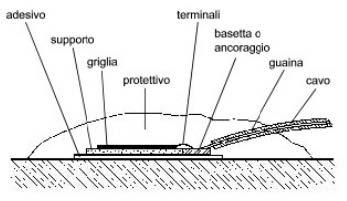
\includegraphics[width=0.5\linewidth]{immagini/1}
			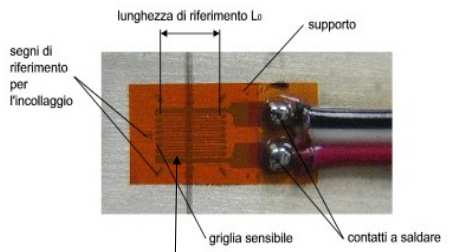
\includegraphics[width=0.5\linewidth]{immagini/2}
			\label{fig:screenshot1}
		\end{figure}
\end{adjustwidth}
\newpage
\subsection{Principio di funzionamento}		
\begin{adjustwidth}{2in}{}						
		Come si valuta una deformazione attraverso ua variazione di resistenza? 
		\[R = \rho {l\over S}\]		
\begin{figure}[H]
	\centering
	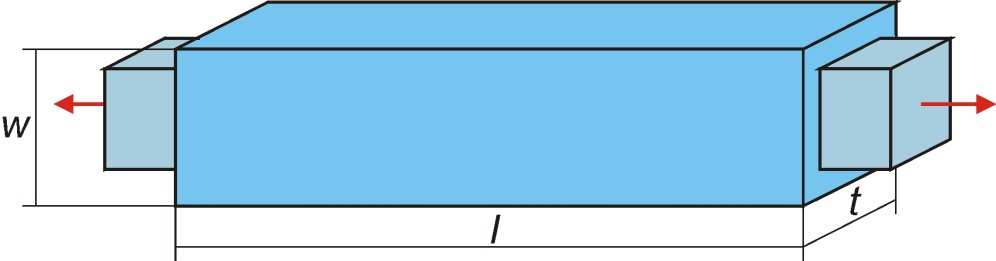
\includegraphics[width=0.5\linewidth]{immagini/3}
	\label{fig:screenshot3}
\end{figure}
		\[R = \rho {l\over wt}\Rightarrow dR = {l\over wt}d\rho + {\rho\over wt}dl - {\rho l\over w^2t}dw - {\rho l\over wt^2}dt\]	
		\[{dR\over R} = {d\rho\over\rho} + {dl\over l} - {dw\over w} -{dt\over t}\]	
		Dove si individuano le deformazioni longitudinali:
		\[\varepsilon_l = {dl\over l}\] 
		E quelle trasversali, esprimibili secondo quelle longitudinali attraverso il modulo di Poisson $\nu$: 
		\[\varepsilon_t = {dt\over t} = -\nu\varepsilon_l \hspace{1cm}
		\varepsilon_w = {dw\over w} = -\nu\varepsilon_l \]
		Per cui: 
		\[{dR\over R} = {d\rho\over\rho} + (1+2\nu)\varepsilon_l\]
		Introduco il fattore di taratura dell'estensimetro come: 
		\[K = \dfrac{dR/R}{\varepsilon_l} = \underbrace{\dfrac{d\rho/\rho}{\varepsilon_l}}_{\text{Effetto piezoresistivo}} + \underbrace{(1+2\nu)}_{\text{Effetto geometrico}}\]
		In modo che: 
		\[{\Delta R\over R} = K\varepsilon_l\]
		È 'effetto piezoresistivo che permette di misurare una variazione di resistenza con la deformazione, mentre l'effetto geometrico dipende invece dal solo modulo di Poisson $\nu$ del materiale. 
		
		Se l’effetto piezoresistivo fosse
		nullo si avrebbe $ K\approx1.6 $.
		
		In realtà il fattore K calcolato
		sperimentalmente per gli estensimetri
		da applicare su acciaio o alluminio
		è circa pari a 2.  
\end{adjustwidth}
\newpage
\subsection{Estensimetri a semiconduttore}		
\begin{adjustwidth}{2in}{}			
		Gli estensimetri a semiconduttore sfruttano proprio l'effetto piezoresistivo, infatti la piezoresistività aumenta in funzione del drogaggio del semiconduttore: $ K\approx200 $ tipo \textit{p}, $ K\approx-125 $ tipo \textit{n}.\newline
		
		Trascurando l'effetto geometrico si ha:
		\[{d\rho\over\rho} = \pi_l\sigma_l + \pi_t\sigma_t\]
		Con $ \pi_l, \pi_t$ rispettivamente coefficienti di piezoresistività longitudinale e trasversa, dipendenti dal tipo di drogaggio. 
		La sensibilità dell'estensimetro è tale per cui, essendo:
		\[{\Delta R\over R} = K\varepsilon \Rightarrow S = {d\varepsilon\over R} = KR\]
		Per ottenere allora un estensimetro più sensibile a parità di resistività si possono percorrere due vie, quella per la quale si sceglie una resistenza maggiore ma di contro si ottiene una maggiore dimensione dell'estensimetro; oppure quella per la quale si sceglie un alto valore di K, e quindi estensimetri piezoresistivi, che di contro hanno un'alta sensibilità alla temperatura. Gli estensimetri piezoresistivi sono miniaturizzabili. \newline 
		
		Come si aumenta la resistenza? 
		\[R = \rho {l\over S}\]
		A resistività costante, si può scegliere un aumento di lunghezza o una diminuzione di sezione.
\begin{figure}[H]
	\centering
	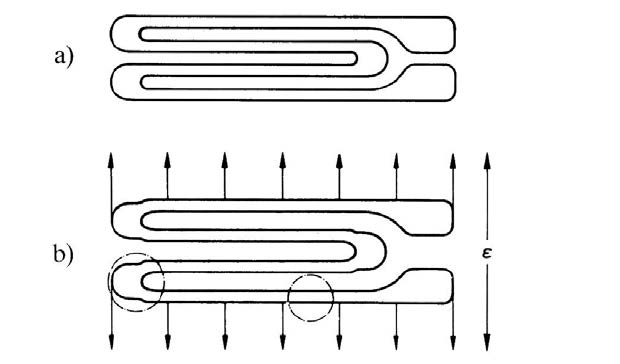
\includegraphics[width=0.5\linewidth]{immagini/4}
\end{figure}
		L'errore in questo caso sta nel fatto che il sensore ottiene una misura mediata e non puntuale come la si vorrebbe, allora verrebbe automatico diminuirne le dimensioni, ma se $l\downarrow\Rightarrow$R$\downarrow$ ed S$\downarrow$, cosa assolutamente non auspicabile, e quindi si aumentano le dimensioni con una configurazione a griglia, che mantenga elevata la sensibilità ma permetta ugualmente una misura puntuale, locale. 
\newpage		
		Una configurazione a griglia però è succube di errori dovuti al posizionamento degli assi delle resistenze secondo direzioni trasversali non oggetto della misurazione: 
\begin{figure}[H]
	\centering
	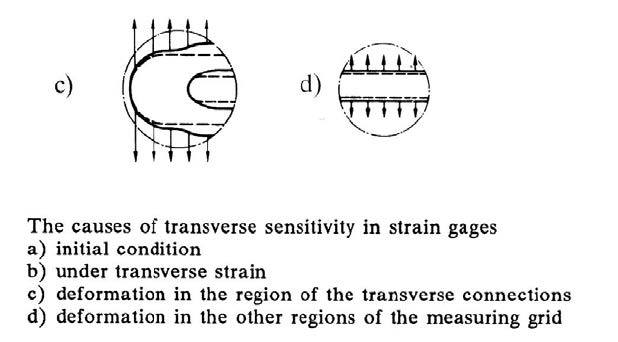
\includegraphics[width=0.5\linewidth]{immagini/5}
\end{figure}
		Per ovviare a questo inconveniente si ingrandisce la sezione che non si vuole misurare, in questo modo, attraverso la legge della resistenza, si nota subito che all'aumentare della sezione si misura una variazione di resistenza sempre minore: si sono resi trascurabili gli effetti sull'estensimetro delle deformazioni traversali. 
\end{adjustwidth}
%\newpage
\subsubsection{Schemi di funzionamento}		
\begin{adjustwidth}{2in}{}	
\begin{figure}[H]
	\centering
	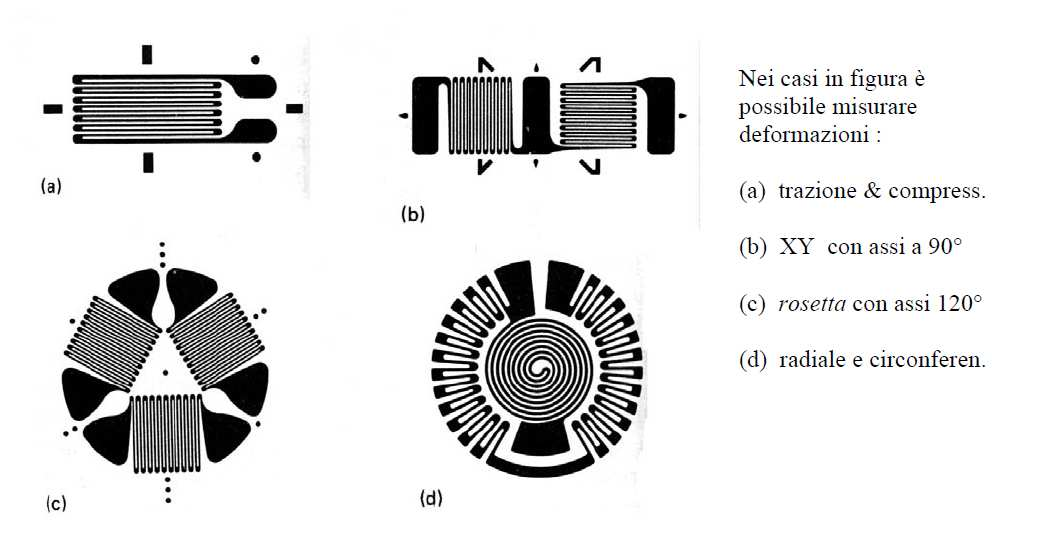
\includegraphics[width=1\linewidth]{immagini/6}
\end{figure}		
		Valori tipici di resistenza base variano tra $100\div1000\Omega$. 
\end{adjustwidth}
\newpage
\subsection{Grandezze di influenza}		
\begin{adjustwidth}{2in}{}
		Un grande problema per gli estensimetri è dato dalle grandezze di influenza, all'interno del trasduttore cioè, oltre a misurare una variazione di resistenza dovuta alla deformazione, si misura una variazione di resistenza dovuta anche alla temperatura, che se fosse ambientale potrebbe essere mantenuta sotto controllo, ma dato che una misura di resistenza non avviene senza un'alimentazione e quindi un passaggio di corrente, si manifesta come un inevitabile autoriscaldamento per effetto Joule.  
		\[{\Delta R\over R}_{\text{finale}} = {\Delta R\over R}_{\Delta T} + {\Delta R\over R}_{\varepsilon}\]
		I contributi che si identificano non appena sussiste uno squilibrio di temperatura sono:
		\begin{itemize}
			\item Effetto Joule 
			\[{\Delta R'\over R}=\alpha\Delta T\]
			\item Deformazione della griglia dell'estensimetro
			\[{\Delta l'\over l} = \beta'\Delta T\]
			\item Deformazione del materiale al di sotto dell'estensimetro
			\[{\Delta l''\over l} = \beta''\Delta T\]
		\end{itemize}
		L'effetto che si ottiene è perciò quello di un allungamento differenziale tra la griglia dell'estensimetro ed il materiale del pezzo sottostante:
		\[{\Delta l\over l} = (\beta'- \beta'')\Delta T\]
		Che porta ad un'ulteriore variazione di resistenza misurata, che si aggiunge a quella già ottenuta per effetto Joule. 
		\[{\Delta R''\over R}=K(\beta'- \beta'')\Delta T\]
		Un uscita si ha così una somma di effetti voluti, oggetto della misurazione, ed effetti non voluti dovuti alle grandezze d'influenza:
		\[{\Delta R\over R} + {\Delta R\over R}_T\]
		\[K\varepsilon + \left[\alpha + K(\beta'- \beta'')\Delta T\right]\]
		 \textbf{Come si tengono a bada le grandezze d'influenza?}
		 \begin{itemize}
		 	\item Si ricorre ad un \underline{Ponte di Wheatstone} a due estensimetri, uno attivo che misurerà la deformazione in oggetto, a cui viene collegato sul ramo contiguo un estensimetro compensatore; questo, non essendo soggetto alla deformazione darà la sua quota parte dovuta alle grandezze di influenza.
\begin{figure}[H]
	\centering
	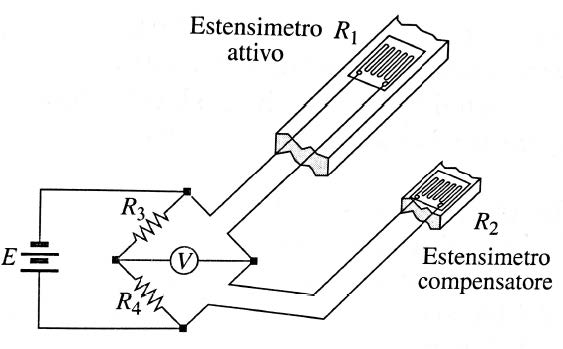
\includegraphics[width=0.3\linewidth]{immagini/7}
	\label{fig:7}
\end{figure}
		 	\[{\Delta V\over E} = {1\over4}\left({\Delta R_1\over R} - {\Delta R_2\over R}\right) = {1\over4}\left(\underbrace{{\Delta R_{\text{misurato}}\over R} + {\Delta R_{\text{influenza}}\over R}}_{{\Delta R_1\over R}} - \underbrace{{\Delta R_{\text{influenza}}\over R}}_{{\Delta R_2\over R}}\right) \]
		 	Col Ponte di Wheatstone si compensano automaticamente le variazioni di resistenza.
		 	
		 	\item Equivalentemente si può ricorrere ad \underline{estensimetri autocompensati} in temperatura, dove si minimizza il contributo dovuto alla temperatura scegliendo opportunamente, per
		 	ogni materiale da studiare l’estensimetro che meglio approssima la relazione:
			\[\left[\alpha + K(\beta'- \beta'')\Delta T\right] = 0\]
			Questa tipologia di estensimetri annulla gli effetti termici ma è utilizzabile per specifici materiali e affinché valgano le ipotesi di misurare bassi $\Delta T$, le variazioni di temperatura devono essere contenute $\sim20\degree C$. 
	\begin{figure}[H]
		\centering
		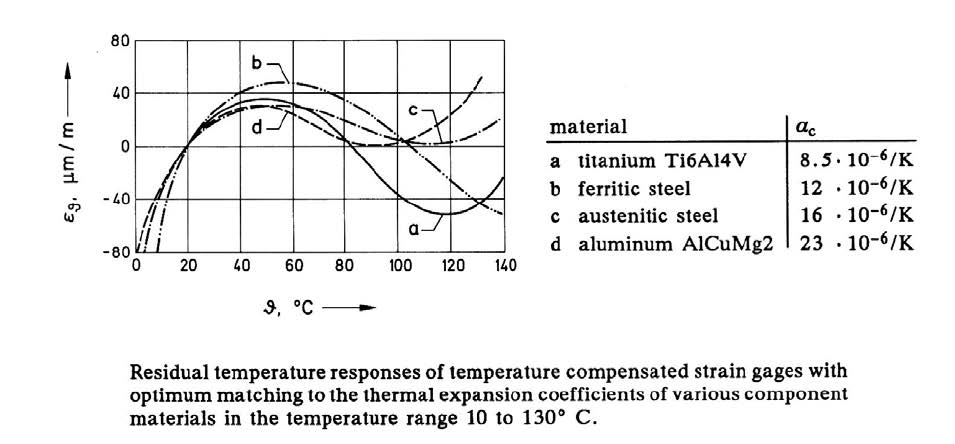
\includegraphics[width=0.5\linewidth]{immagini/8}
		\label{fig:8}
	\end{figure}	
		 \end{itemize}
\paragraph{Esempio}\mbox{} \\ 
		 L'unità di misura della deformazione "non esiste", dato che questa è adimensionale, nelle applicazioni meccaniche, dato che le deformazioni misurate sono dell'ordine dei micrometri, si usa spesso la quantità: 
		 \[{\mu m\ m} = 10^{-6} = \mu\varepsilon = ~ \text{microstrength}\] 
		 In questo modo, piuttosto che dire la deformazione è pari a $100\cdot10^{-6}$ si dice che la deformazione è pari a $100\mu\varepsilon$.\newline 
		 
		 Ora, avendo una deformazione pari a $100\mu\varepsilon$ ed un estensimetro di resistenza $120\Omega$, la variazione di resistenza è pari a: 
		 \[{\Delta R\over R} = K\varepsilon \Rightarrow \Delta R = RK\varepsilon = 120\Omega \cdot 2 \cdot 100\cdot10^{-6} = 0.024\Omega = 24m\Omega\]
		 
		 Per effettuare la misura si utilizzano o il metodo di zero, valutando quindi la resistenza quando $\Delta V=0$, oppure il metodo a deflessione, quest'ultimo risulta il più utilizzato per misurare una deformazione variabile nel tempo.  
\end{adjustwidth}
\newpage
\section{Misure di Forza}		
\begin{adjustwidth}{2in}{}	 
		 Per misurare una forza si utilizzano le celle di carico, queste sono costituite da un elemento elastico (trasduttore primario) che converte forza e torsione in deflessione o deformazione ed uno o più trasduttori secondari che convertono la deflessione o la deformazione in un'altra grandezza fisica generalmente di natura elettrica.
		 \[F~\text{o}~M\rightarrow\boxed{\text{trasduttore}}\rightarrow\Delta V\]
		 \[F~\text{o}~M\rightarrow\boxed{I}\rightarrow\varepsilon\rightarrow\boxed{II}\rightarrow{\Delta R\over R}\rightarrow\boxed{PW}\rightarrow\Delta V\]
\begin{figure}[H]
	\centering
	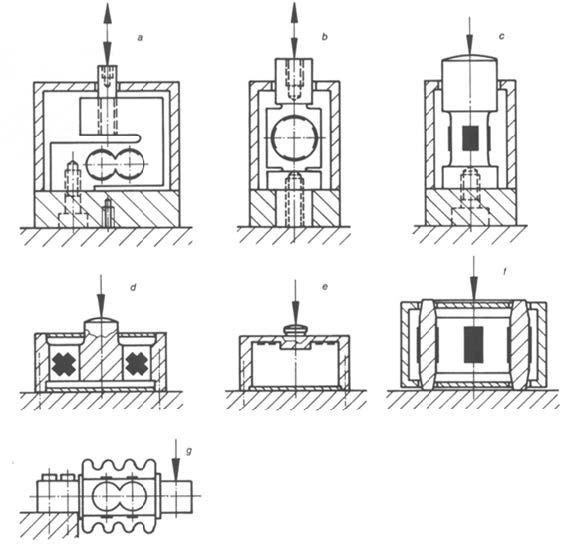
\includegraphics[width=0.5\linewidth]{immagini/9}
	\label{fig:9}
\end{figure}
		 Le celle di carico devono coprire la maggior parte delle applicazioni, per questo se ne trovano delle più svariate dimensioni ma sempre di tre tipologie, o a Trazione o a Flessione o a Taglio.
		 
		 Una cella di carico multicomponente riunisce sotto un unico strumento le tre tipologie appena viste. 
\end{adjustwidth}
%\newpage
\subsection{Criteri di progetto}		
\begin{adjustwidth}{2in}{}			 
		 Come si progetta l'elemento elastico che si deve deformare? Come si progettano i trasduttori? \newline 
		 \textbf{Ipotesi di progetto dell'elemento elastico:}
		 \begin{enumerate}
		 	\item L'applicazione della forza determina una variazione lineare del campo di
		 	deformazioni rilevato dall'estensimetro: si deve rimanere all'interno del limite elastico;
		 	
		 	\item Frequenza di oscillazione propria di valore sufficientemente elevato: si deve evitare la risonanza e l'amplificazione dinamica degli effetti $\omega_n=\sqrt{k/m}\ne\omega_0$;
		 	
		 	\item Sufficiente valore del campo delle deformazioni nella zona di applicazione
		 	degli estensimetri elettrici a resistenza ($ 1000-1700 \mu m/m $ a carico nominale): si devono avere delle dimensioni atte a misurare la deformazione;
		 	
		 	\item Uniformità della distribuzione delle deformazioni nell'area esaminata dagli
		 	estensimetri elettrici a resistenza: la zona di incollaggio deve essere uniforme, senza presenza di microbolle o variazioni delle caratteristiche superficiali del materiale; 
		 	
		 	\item La zona nella quale sono applicati gli estensimetri deve essere quella
		 	dove si manifestano le deformazioni di valore più elevato; 
		 	
		 	\item Realizzazione dell'elemento elastico in un solo pezzo;
		 	
		 	\item Disegno capace di facilitare l'installazione degli estensimetri, l'elemento elastico deve predisporre degli alloggiamenti per l'istallazione degli estensimetri;
		 	
		 	\item Protezione dai sovraccarichi (circa il 200\% del FS e 300-500\% FS rottura
		 	cella): non si vuole superare il limite elastico. 
		 	
		 	\item Modesto spostamento del punto di applicazione della forza dovuto alla
		 	deflessione dell'elemento elastico: non si deve variare la distanza di applicazione della forza; 
		 	
		 	\item Modesti effetti dovuti a variazioni della temperatura di lavoro.
		 	
		 	\item Insensibilità ai carichi trasversali.
		 	
		 	Modificando la dimensione dell'elemento elastico si fa in modo che questo sia deformabile nella zona in cui interessa la misura e indeformabile e rigido dove NON interessa la misura.
		 	\begin{figure}[H]
		 		\centering
		 		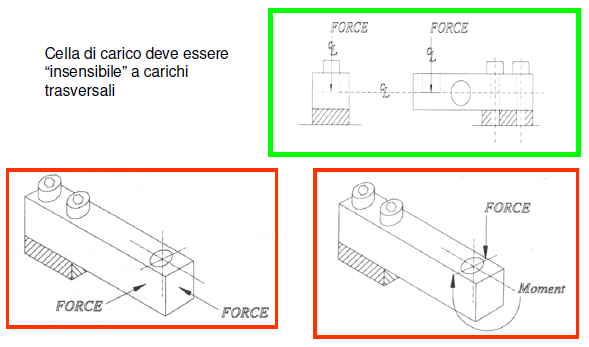
\includegraphics[width=0.5\linewidth]{immagini/screenshot003}
		 		\label{fig:screenshot003}
		 	\end{figure}		 	
		 \end{enumerate}
\end{adjustwidth}
%\newpage
\subsubsection{Eliminazione dell'effetto di carichi trasversali}		
\begin{adjustwidth}{2in}{}	
	 	Per evitare e limitare questi effetti la prima idea che si sviluppa è quella di "insottilire" l'elemento elastico per renderlo più deformabile, ma inevitabilmente sia a taglio che a trazione si romperebbe, si usano allora degli elementi a cedevolezza differenziata, questi infatti nascono dalla necessità di svincolare la cella di carico dalla base e dalla forza applicata. \newline 
	 	
	 	Si usano dei dischi che permettono lo spostamento dell'elemento elastico nella direzione di deformazione interessata dalla misurazione, ma lo bloccano nelle altre direzioni. 
	 	
	 	In figura l'elemento può muoversi $\updownarrow$ ma è impedito in $\leftrightarrow$. 
\begin{figure}[H]
	\centering
	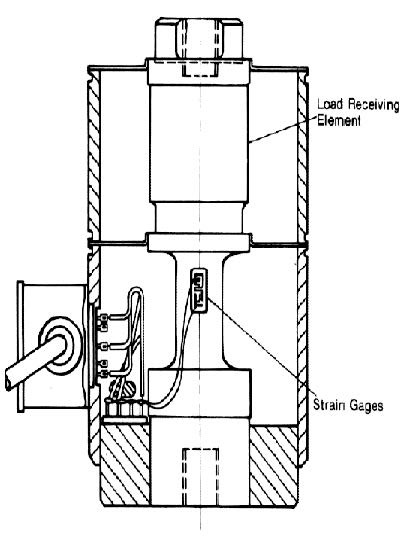
\includegraphics[width=0.2\linewidth]{immagini/10}
	\label{fig:10}
\end{figure}
\newpage
	 	Un'altra misura adottata per limitare gli spostamenti trasversali è l'applicazione di disaccoppiatori. 
	 	
	 	Questi, disaccoppiando la forza svincolano il vincolo che determinerebbe la rottura dell'elemento elastico in modo da non opporsi alla forza indesiderata che subisce. 
	 	
	 	\begin{figure}[H]
	 		\centering
	 		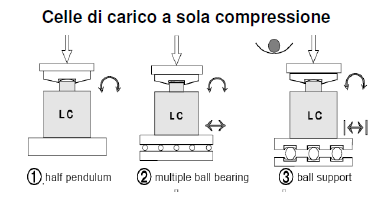
\includegraphics[width=0.5\linewidth]{immagini/screenshot004}
	 		\label{fig:screenshot004}
	 	\end{figure}	 	 
	 	\begin{figure}[H]
	 		\centering
	 		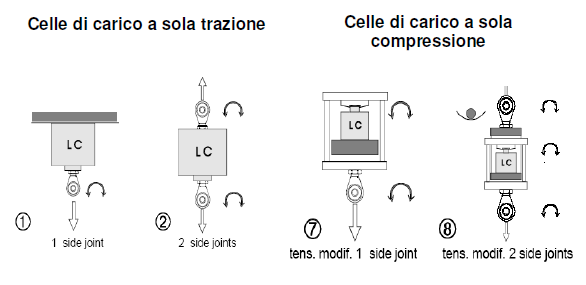
\includegraphics[width=0.5\linewidth]{immagini/screenshot005}
	 		\label{fig:screenshot005}
	 	\end{figure}
\end{adjustwidth}
%\newpage
\subsection{Celle di carico a Trazione e Compressione}		
\begin{adjustwidth}{2in}{}	
	 	L'asse sensibile di questa tipologia di celle di carico è quello verticale, l'elemento elastico si muove $\updownarrow$.  
	 	\begin{figure}[H]
	 		\centering
	 		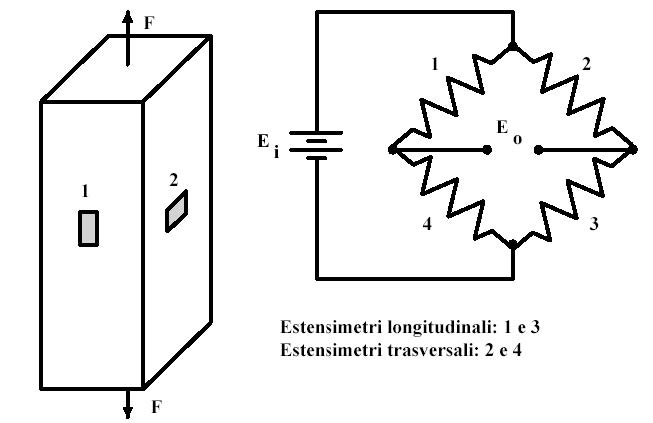
\includegraphics[width=0.3\linewidth]{immagini/11}
	 		\label{fig:11}
	 	\end{figure}	 	
	 	Si schematizza come un parallelepipedo a cui è applicata una forza assiale e si misura una deformazione assiale:
	 	\[\varepsilon_a = {F\over AE} \hspace{1cm} \varepsilon_t = -\nu\varepsilon_a\]
	 	Il collegamento degli estensimetri avviene attraverso il più che collaudato Ponte di Wheatstone, in cui gli estensimetri 1 e 3, opposti, sono quelli sensibili alla deformazione assiale, oggetto della misura: 
	 	\[{\Delta R_1\over R_1} = {\Delta R_3\over R_3} = K\varepsilon_a = K{F\over AE}\]
	 	In questo modo si ottiene un uscita pari a:
	 	\[{\Delta V\over E} = {1\over 2}{\Delta R_1\over R_1} = {1\over 2} K{F\over AE}\]
	 	Ovvero il doppio di quella che si sarebbe ottenuta applicando un solo estensimetro assiale. \newline 
	 	
	 	\textbf{Come si aumenta la sensibilità?} 
	 	
	 	Applicando due estensimetri contigui a 1 e 3 che misurino una variazione opposta a questi e tra di loro contrapposti, 2 e 4. 
	 	
	 	Questi estensimetri ora trasversali misurano la compressione dell'elemento elastico:
	 	\[{\Delta R_2\over R_2} = {\Delta R_4\over R_4} = K\varepsilon_t = -K\nu{F\over AE}\]
	 	L'uscita che si ottiene sarà data infine da:
\end{adjustwidth} 
	 	\[{\Delta V\over E_i} = {1\over 4} \left({\Delta R_1\over R_1} + {\Delta R_3\over R_3} -{\Delta R_2\over R_2} - {\Delta R_4\over R_4}\right) = {1\over 4}\left[2K{F\over AE}-\left(-2K\nu{F\over AE}\right)\right] = {1\over 4} \left[{2KF(1+\nu)\over AE}\right]\]
	 	\[{\Delta V\over E_i} = {KF(1+\nu)\over2 AE}\] 
\begin{adjustwidth}{2in}{}
	 	Invertendo si ottiene: 
	 	\[F = {\Delta V\over E_i}{2 AE\over K(1+\nu)}\]
	 	La sensibilità è:
	 	\[S = {\Delta V\over F} = {K(1+\nu)E_i\over2 AE}\]
	 	Questa dipende:
	 	\begin{itemize}
	 		\item Dalla geometria dell'elemento elastico, ossia dalla sezione assiale $A$.
	 		
	 		$A\downarrow$ implica l'utilizzo di un elemento elastico più piccolo, ma un $A\downarrow$ implica anche una sezione di materiale resistente molto più bassa, ovvero entità minori di forze misurabili. 
	 		
	 		\item Dal materiale scelto per realizzare l'elemento elastico di connessione, ossia $E$ e $\nu$. 
	 		
	 		$E\downarrow$ si ottiene utilizzando materiali dal modulo elastico più marcato, come l'alluminio. 
	
	 		\item Dagli estensimetri utilizzati, ossia dal fattore di taratura $K$. 
	 		
	 		Un $K\uparrow$ si può ottenere tramite l'impiego di estensimetri piezoresistivi. 
	 		
	 		\item Dalla tensione di alimentazione utilizzata per il Ponte di Wheatstone $E_i$. 
	 		
	 		Una $E_i \uparrow$ implica però un rischio maggiore di incorrere nell'effetto Joule. 
	 	\end{itemize} 
 		Notare tuttavia come sia impossibile ottenere una sensibilità unitaria ed intera perché questa sarà sempre funzione del modulo di Poisson, in ogni caso sarà sempre maggiore di quella ottenuta utilizzando solamente due estensimetri. \newline

	 	La portata massima della cella di carico dipende così dal limite elastico del
	 	materiale $\sigma_F$: 
	 	\[\left(\Delta V\over E_i \right)_{\text{max}}= {K\sigma_F(1+\nu)\over2 AE}\] 
	 	Con: 
	 	\[F_{\text{max}} = A\sigma_F\]
	 	All'aumentare della sezione trasversale aumenta si il valore della portata massima, ma diminuisce inevitabilmente la sensibilità. \newline 
	 	
	 	La sensibilità di una cella di carico si misura:
	 	\[S = {\Delta V\over F} = \left[mV\over N\right]\] 
	 	Generalmente a catalogo la sensibilità di una cella di carico viene espressa secondo una sensibilità nominale definita come $ mV/V $ a Fondo Scala (FS) ed
	 	un valore tipico è $ 2mV/V $.\newline 
	 	
	 	Per ottenere la sensibilità propria della cella di carico a partire da quella nominale: 
	 	\[ \left[{mV\over \cancel{V}}\cdot{\cancel{E_i}\over FS}\right] = \left[mV\over N\right] \]
	 	E quindi l'operazione da effettuare è la seguente: 
	 	\[ S = S_n\cdot {E_i\over FS}\]
	 	Moltiplicando per un fattore 1000 se si vuole una sensibilità in \(\left[V\over N\right]\)
	 	E se si volesse misurare forze e masse nell'ordine delle tonnellate? Dato che si usa dimensionarlo con una sezione assiale 5 volte maggiore della sezione trasversale per evitare effetti di bordo dovuti all'anisotropia tra trazione e compressione, si costruirebbero elementi elastici enormi, ciò che si fa è distribuire e riequilibrare la forza tra più elementi elastici e la misura in oggetto diventa possibile attraverso 4 ponti di Wheatstone ed un circuito sommatore. 
\begin{figure}[H]
	\centering
	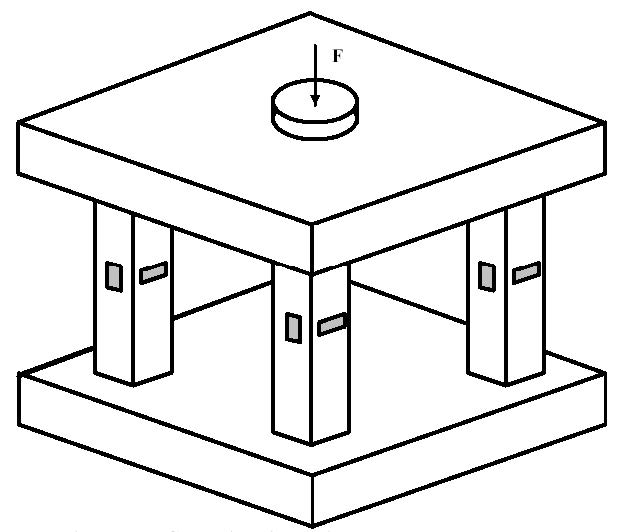
\includegraphics[width=0.2\linewidth]{immagini/12}
	\label{fig:12}
\end{figure}
\end{adjustwidth}
%\newpage
\subsection{Celle di carico a Flessione}		
\begin{adjustwidth}{2in}{}	
	 	Sono costituite da una lamina incastrata che studia e misura la deformazione a flessione. 
	 	
	 	Gli estensimetri si mettono sempre nella zona di massima deformazione, si collocano il più possibile vicino al vincolo d'incastro. 
\begin{figure}[H]
	\centering
	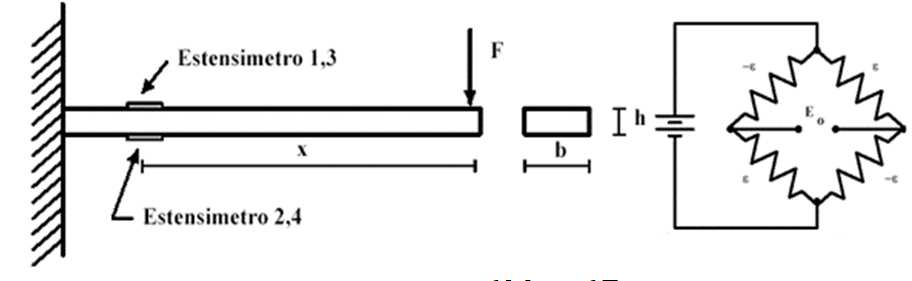
\includegraphics[width=0.5\linewidth]{immagini/13}
	\label{fig:13}
\end{figure}
	 	Come si è visto quando si è trattato il Ponte di Wheatstone, si incollano 1, 3 sopra e 2, 4 sotto, in modo che misurino deformazioni uguali sui rami opposti e opposte sui rami contigui:
	 	\[\varepsilon_1 = \varepsilon_3 = -\varepsilon_2 = -\varepsilon_4 = {6M\over EA} = {6Fx\over Ebh^2}\] 
	 	In cui $b$ ed $h$ sono rispettivamente la larghezza e l'altezza della lamina, $x$ è la distanza del punto di applicazione della forza dal punto medio dell'area
	 	esaminata dagli estensimetri ed $E$ è il modulo di Young del materiale costituente la lamina. 
	 	
	 	\[{\Delta R_1\over R_1} = {\Delta R_3\over R_3} = -{\Delta R_2\over R_2} = -{\Delta R_4\over R_4} = K{6Fx\over Ebh^2}\]
	 	In questo modo si ottiene, al contrario della cella a trazione dove non si poteva eliminare il contributo dato da Poisson, una sensibilità intera: 
	 	\[{\Delta V\over E_i} = K{6Fx\over Ebh^2}\]
	 	Invertendo: 
	 	\[ F = {\Delta V\over E_i}{Ebh^2\over K6Fx}\]
	 	Per cui: 
	 	\[S = {E_0\over F} = {K6FxE_i\over Ebh^2} \]
\newpage
	 	La sensibilità dipende perciò da:
	 	\begin{itemize}
	 		\item La geometria scelta per la lamina, attraverso $b$ ed $ h $. 
	 		
	 		$A\downarrow$ e quindi scegliendo una mensola più sottile si giunge tuttavia prima allo snervamento. 
	 		
	 		\item Il modulo elastico del materiale utilizzato per la lamina, $ E $.
	 		
	 		$E\downarrow$ scegliendo magari un materiale come l'alluminio. 
	 		
	 		\item Il posizionamento del punto di applicazione del carico rispetto a dove sono
	 		stati applicati gli estensimetri, $x$. 
	 		
	 		$x\uparrow$ si devono scegliere punti di applicazione e rilevamento sufficientemente lontani. 
	 		
	 		\item La sensibilità degli estensimetri, K. 
	 		
	 		Scegliendoli ad esempio piezoresistivi. 
	 		
	 		\item Il valore della tensione di alimentazione scelta per il ponte, $E_i$. 
	 		
	 		Cercando di limitare quanto possibile l'autoriscaldamento. 
	 	\end{itemize}		
 		Le celle di carico a flessione sono di loro natura più sensibili di quelle a trazione/compressione, in queste ultime infatti erano stati usati due estensimetri per misurare la deformazione assiale e due estensimetri per quella trasversale, per cui c'era di mezzo un Poisson, mentre in questo caso tutti e quattro gli estensimetri misurano la stessa tipologia deformazione a flessione. 
 	
 		Applicando gli estensimetri in prossimità dell'incastro, come si è anticipato, questi percepiscono il momento flettente massimo:
 		\[\sigma_{\text{max}} = E\varepsilon \hspace{1cm} \varepsilon={6Fx\over Ebh^2} \hspace{1cm} F_{\text{max}} = {\sigma_{\text{max}}bh^2\over6x}\]
 		In cui $ \sigma_{\text{max}} $ è il limite elastico del materiale.\newline 

 		Se l'obbiettivo è quello di ottenere un elevato campo di misura, o si diminuisce la distanza $x$ di applicazione del momento o si aumenta la sezione resistente, ma entrambe portano ad un crollo della sensibilità.  
 		
 		\[\left(\Delta V\over E_i \right)^{\text{flessione}}_{\text{max}}={K\sigma_{\text{max}}\over E}\hspace{1cm}\text{VS}\hspace{1cm}\left(\Delta V\over E_i \right)^{\text{trazione}}_{\text{max}}= {K\sigma_{\text{max}}(1+\nu)\over2 AE}\] 	
 		\begin{figure}[H]
 			\centering
 			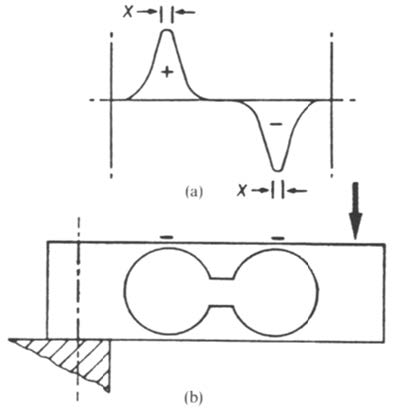
\includegraphics[width=0.5\linewidth]{immagini/14}
 			\label{fig:14}
 		\end{figure} 
\newpage			
 \paragraph{Lamina Incastrata}
 		\begin{itemize}[label=\textcolor{green}{\cmark}]
 			\item Elevata sensibilità;
 			
 			\item Presenza di due superfici nelle quali si manifestano deformazioni di segno
 			opposto;
 			
 			\item Applicazione facile degli estensimetri;
 			
 			\item Se lo spessore della lamina è sufficientemente piccolo si ottengono evidenti
 			vantaggi per la compensazione degli effetti indotti dalla temperatura: gli estensimetri subiscono lo stesso $\Delta T$ e il contributo delle grandezze di influenza si sottrae.
 		\end{itemize}
 		
 		\begin{itemize}[label=\textcolor{red}{\xmark}]
 			\item La conversione della forza applicata in momento flettente viene effettuata su
 			tutta la lamina e non solamente nella zona di applicazione degli estensimetri.
 			
 			Per ovviare a questo inconveniente si rastrema l'elemento nella zona d'applicazione degli estensimetri e lo si ingrandisce nel punto di applicazione della forza, in questo modo a sentire la deformazione sarà soltanto la zona di applicazione degli estensimetri. 		
 	\begin{figure}[H]
 		\centering
 		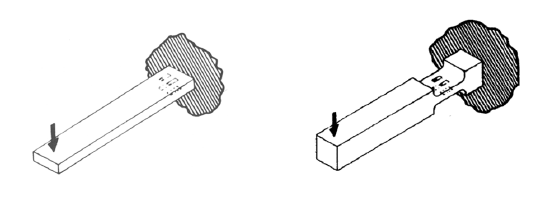
\includegraphics[width=0.5\linewidth]{immagini/screenshot006}
 		\label{fig:screenshot006}
 	\end{figure}			
 			La deformazione variabile su tutto il pezzo si contiene ricordando inoltre che questa:
 			\[\varepsilon\sim{x\over bh^2}\]
 			Variando inevitabilmente la $x$, si può manipolare $b$  per ottenere sempre un rapporto costante, si fa in modo che:
 			\[{x\over b}=cost\]
 			Rastremando il pezzo.
 			\begin{figure}[H]
 				\centering
 				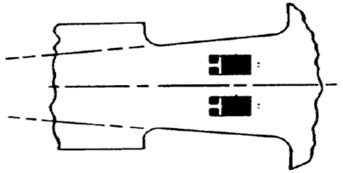
\includegraphics[width=0.3\linewidth]{immagini/15}
 				\label{fig:15}
 			\end{figure}			
 			\item La frequenza propria è tendenzialmente di valore contenuto.
 			
 			Per ovviare a questo problema si sceglie di forare longitudinalmente il pezzo: 
 			\[\omega_n=\sqrt{k\over M}\]
 			Come $M\downarrow, \, \omega_n\uparrow$ e si aumenta la banda passante del sistema. 
 			\begin{figure}[H]
 				\centering
 				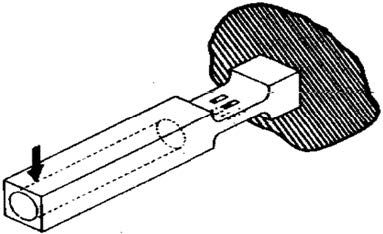
\includegraphics[width=0.3\linewidth]{immagini/16}
 				\label{fig:16}
 			\end{figure}
 		\end{itemize}
 		Inoltre, per ovviare problemi di compensazione, se scelgono geometrie particolarmente studiate come quella a S, dove la zona di massima deformazione, e quindi dove si applicano gli estensimetri, è quella centrale, e non più le lamine, le quali, a flessione, longitudinalmente possono andare contemporaneamente a compressione e a trazione sui rami contigui.
 		\begin{figure}[H]
 			\centering
 			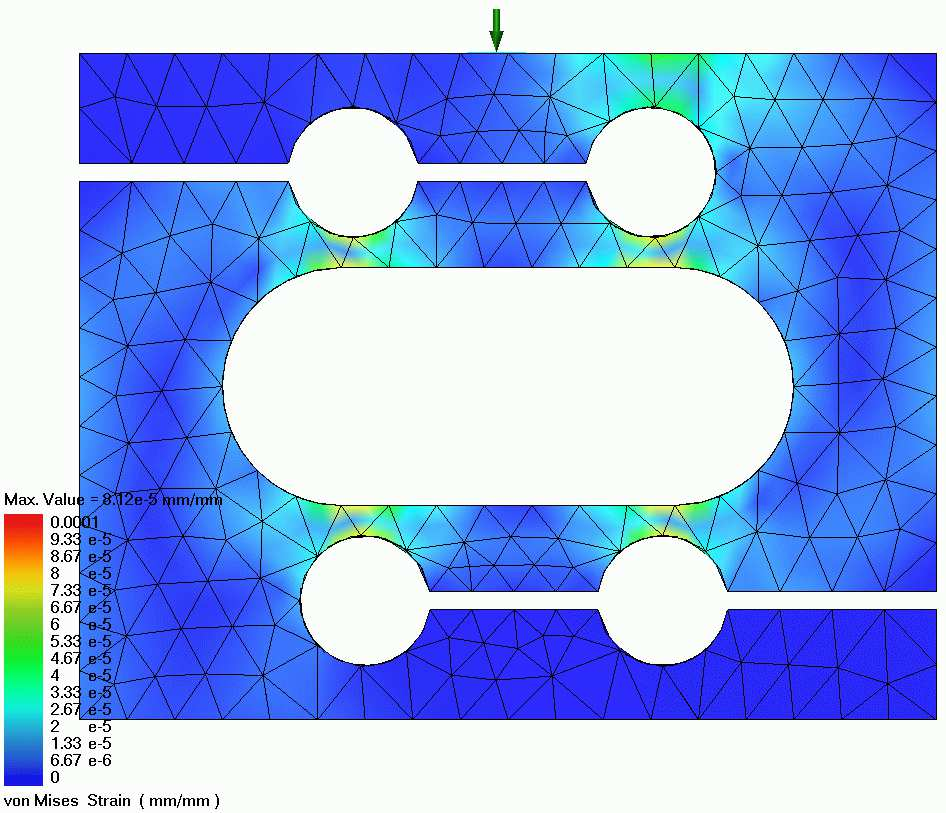
\includegraphics[width=0.5\linewidth]{immagini/17}
 			\label{fig:17}
 		\end{figure}
\end{adjustwidth}
%\newpage
\subsection{Celle di carico a Taglio}		
\begin{adjustwidth}{2in}{}	
 		La sezione dell'elemento elastico di una cella di carico a taglio è nient'altro che una trave a doppia T, dove gli estensimetri vengono posti a 45\degree esattamente sull'asse neutro di tale sezione in modo da non sentire alcuna influenza delle sollecitazioni a flessione, ma solo la massima della sollecitazione di taglio. 
\begin{figure}[H]
	\centering
	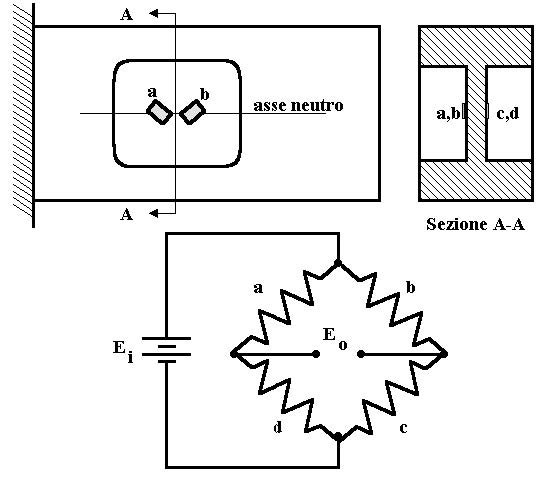
\includegraphics[width=0.3\linewidth]{immagini/18}
	\label{fig:18}
\end{figure}
\begin{figure}[H]
	\centering
	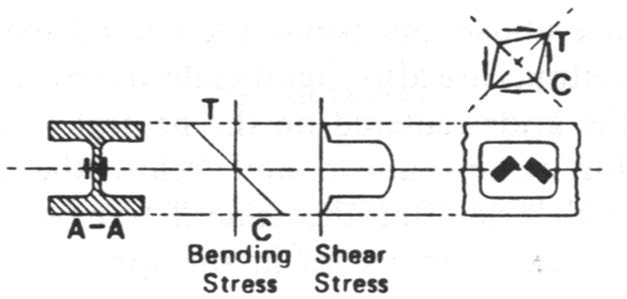
\includegraphics[width=0.3\linewidth]{immagini/19}
	\label{fig:19}
\end{figure}
 		\begin{itemize}[label=\textcolor{green}{\cmark}]
 			\item Modesto ingombro trasversale;
 			\item La massa dell'equipaggio mobile del trasduttore è di valore contenuto;
 			\item Intrinseca compattezza e rigidezza;
 			\item Riescono a rilevare fenomeni rapidamente variabili nel tempo (2-20kHz), alta variabilità dell'applicazione della forza;
 			\item Estensimetri protetti. 			
 		\end{itemize}
 	
 		\begin{itemize}[label=\textcolor{red}{\xmark}]
 			\item Non agevole applicazione degli estensimetri;
 			\item La portata minima non può essere ridotta oltre un certo limite poiché la
 			sezione equipaggiata con estensimetri non può essere troppo sottile per
 			evitare fenomeni di instabilità;
 			\item Non completa uniformità del campo delle deformazioni al di sotto degli
 			estensimetri.
 			
 			Per risolvere questo problema si ricorre sia all'utilizzo di rosette estensimetriche che alla scelta di una configurazione più compatta. 			
 			\begin{figure}[H]
 				\centering
 				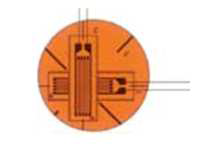
\includegraphics[width=0.3\linewidth]{immagini/screenshot007}
 				\label{fig:screenshot007}
 			\end{figure}		 
 		\end{itemize}
\end{adjustwidth}
%\newpage
\subsection{Celle di carico a Torsione}		
\begin{adjustwidth}{2in}{}	
 		In che modo e che tipo di elemento elastico misura la deformazione a torsione? \newline 
 		
 		I torsiometri possono essere installati sia su alberi fissi che su alberi rotanti, sia vincolando l'albero che interrompendolo. \newline 
 		
 		Un torsiometro è schematizzabile come un primo trasduttore della figura un elemento elastico costituto da un albero di sezione circolare, ed un secondo trasduttore costituito da estensimetri elettrici a resistenza.  		
 		\begin{figure}[H]
 			\centering
 			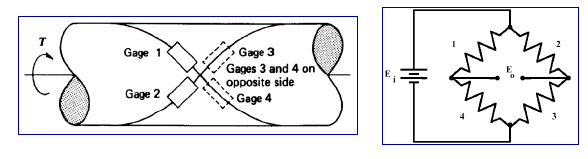
\includegraphics[width=0.5\linewidth]{immagini/screenshot008}
 			\label{fig:screenshot008}
 		\end{figure} 	 		
 		Gli estensimetri così posti, sulla superficie misurano, a 45\degree ad elica, la massima deformazione alla massima sensibilità possibile. \newline 
 		
 		La torsione alla Jourasky per sezione circolare era: 
 		\[\tau_{\text{max}} = {TD\over2J} = {16T\over\pi D^3}\]
 		In cui $T$ è la torsione applicata, $D$ è il diametro dell'albero, $J$ è il momento d'inerzia polare della sezione circolare, e  $\tau_{\text{max}}$ è la tensione tangenziale massima. \newline 
 		
 		Per un albero circolare sollecitato a pura torsione, le tensioni normali sono nulle: 
 		\[\sigma_x = \sigma_y = \sigma_z = 0\]
 		Dunque, le tensioni principali saranno: 
 		\[\sigma_1 = - \sigma_2 = \tau_{\text{max}} = {16T\over\pi D^3}\]
 		\[\varepsilon_1 = \dfrac{(\sigma_1-\nu\sigma_2)}{E} = {16T\over\pi D^3}\left(1+\nu\over E\right)\]
 		\[\varepsilon_2 = \dfrac{(\sigma_2-\nu\sigma_1)}{E} = -{16T\over\pi D^3}\left(1+\nu\over E\right)\]
 		\[{\Delta R_1\over R_1} = -{\Delta R_2\over R_2} = {\Delta R_3\over R_3}  = - {\Delta R_4\over R_4}  =K{16T\over\pi D^3}\left(1+\nu\over E\right) \]
 		Allora dal ponte di Wheatstone:
 		\[ {\Delta V\over E_i} =K{16T\over\pi D^3}\left(1+\nu\over E\right) \]
 		Invertendo, la torsione è pari a:
 		\[ T = {\Delta V\over E_i} \dfrac{\pi D^3E}{16(1+\nu)K}\]
 		E la sensibilità è: 
 		\[S = K{16\over\pi D^3}\left(1+\nu\over E\right)E_i\]
 		Questa dipende:
 		\begin{itemize}
 			\item Dalla geometria scelta per l'albero, ovvero dal
 			diametro D: D$\downarrow$ S$\uparrow$;
 			
 			\item Dal materiale costituente l'albero, ossia dal modulo elastico $ E $ e dal modulo di Poisson $\nu$;
 			
 			\item Dagli estensimetri utilizzati, ossia dal fattore di
 			taratura $ K $;
 			
 			\item Dalla tensione di alimentazione $E_i$ applicata al ponte.	
 		\end{itemize}
 	
 		Il campo di misura è anche qui dato dalla tensione massima ammissibile che l'albero è in grado di sopportare: 
 		\[T_{\max} = {\pi D^3\over 16}\sigma_{\text{max}}\] 
 	 	Per cui sostituendo: 
 	 	\[\left(E_0\over E_i\right)_{\max} = K\left(1+\nu\over E\right)\sigma_{\text{max}}\]
 	 	E dipende da:
 	 	\begin{itemize}
 	 		\item Dal diametro $D$ dell'elemento elastico;
 	 		\item Dal limite elastico a torsione del materiale scelto; 
 	 	\end{itemize}  	
\paragraph{Cella Differenziale} \mbox{} \\ 
  		Questa cella di carico permette la misurazione della torsione senza l'utilizzo di estensimetri.  		
  		\begin{figure}[H]
  			\centering
  			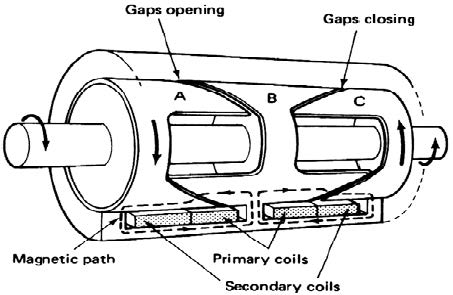
\includegraphics[width=0.5\linewidth]{immagini/20}
  			\label{fig:20}
  		\end{figure}  		
  		È costituita da una barra di torsione (elemento elastico) realizzato in materiale non ferromagnetico a cui vengono applicati tre elementi di materiale ad alta permeabilità magnetica, dei traferri (A, B, C) opportunamente distinti e distinguibili a cui a loro volta sono applicati avvolgimenti primari e secondari. \newline 
  		
  		Dando la stessa intensità di corrente sui circuiti primari si viene a formare un circuito che senza deformazione in atto è simmetrico. 
  		
  		Ricordando che la mutua induzione dipende dal numero di spire degli avvolgimenti e dalla permeabilità magnetica, come la torsione prende luogo, viene a crearsi tra le separazioni dei tre elementi rispettivamente un gap, un allontanamento e dall'altro lato un contatto, un avvicinamento. Il gap determina spazio vuoto, quindi aria che intercorre ed una variabilità della permeabilità magnetica: in questo modo ci si accorge che sta avvenendo deformazione da torsione. \newline 
  		
  		\begin{itemize}
  			\item \(V_{AB} - V_{BC} = 0 \) Assenza di torsione;
  			\item \( V_{AB}\downarrow ~ V_{BC}\uparrow ~ \Rightarrow \Delta V<0 \circlearrowright\) AB si allontana e BC si avvicina;
  			\item \( V_{AB}\uparrow ~ V_{BC}\downarrow ~ \Rightarrow \Delta V>0 \circlearrowleft\) AB si avvicina e BC si allontana;
  		\end{itemize}
  		
  		Infine, a valle del trasduttore uscirà un segnale la cui intensità sarà proporzionale al valore della torsione e la fase dipenderà dalla direzione della stessa.  
  		
\paragraph{Torsiometro Ottico I}\mbox{} \\ 
  		Due identici dischi del tipo ad encoder angolare incrementale sono posti agli
  		estremi dell'albero di torsione. 
  		\begin{figure}[H]
  			\centering
  			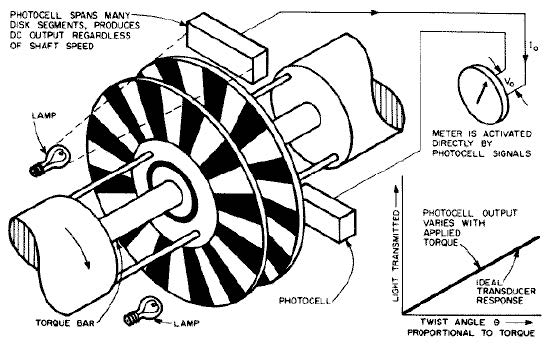
\includegraphics[width=0.5\linewidth]{immagini/21}
  			\label{fig:21}
  		\end{figure}  
  		Ogni disco - intervallato da zone nere e zone trasparenti- è solidale all'albero, tra i due dischi è posto un alberino dal diametro molto più contenuto rispetto a quello esterno che si deformerà e accentuerà la deformazione, si predispongono poi un emettitore di luce ed un foto-rivelatore connesso ad un microamperometro, questo rileverà l'output delle fotocellule. \newline 
  		
  		A riposo, in assenza di torsione, i dischi sono sfasati esattamente della metà, l'area di ricopertura è esattamente pari al 50\%, la quantità di luce che traspare è esattamente la metà del totale. 
  		
  		Appena questo torsiometro ottico viene messo in rotazione relativa dalla torsione, le bande nere si allontanano $ \rightleftarrows $ e l'intensità luminosa  aumenta, se invece la rotazione relativa è invertita le bande nere si sovrappongono a quelle trasparenti $ \leftrightarrows $ e l'intensità luminosa diminuisce.  
  		
\paragraph{Torsiometro Ottico II}\mbox{} \\ 
  		Ciascun estremo della barra di torsione è equipaggiato con marker riflettenti
  		che sono illuminati da luce collimata.
\begin{figure}[H]
	\centering
	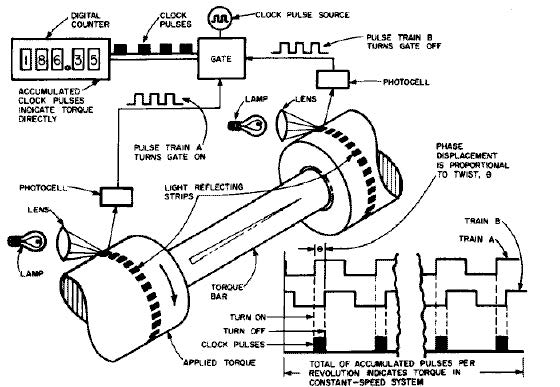
\includegraphics[width=0.5\linewidth]{immagini/22}
	\label{fig:22}
\end{figure}
  		Questo tipo di torsiometro è prettamente utilizzata per alberi in movimento perché garantisce assenza di contatti tra le parti, i cavi di misurazione sono collegati al sistema di misura e non all'oggetto della misurazione. \newline 
  		
  		Anche in questo caso l'albero dal diametro minore è indotto a deformarsi, mentre i diametri maggiori sulla circonferenza sono intervallati da tacche nere e riflettenti. \newline 
  		
  		Una luce fissa al telaio viene collimata da una lente ad incidere su di una tacca per volta, in questo modo durante la rotazione la fotocellula legge una sequenza di ON/OFF, ovvero un'onda quadra che non dà la misura della torsione ma misura solo la presenza della luce. 
  		
  		Per luce riflessa dalla tacca l'onda quadra si accede, per luce assorbita dalla tacca l'onda quadra si spegne. \newline 
  		
  		In assenza di torsione i segnali sono in fase e l'uscita è nulla, in presenza di torsione viene invece a crearsi una variazione dell'output in funzione dello sfasamento dei due segnali, il sistema misura così il tempo tra gli sfasamenti. 
  		
  		Il segnale acquisito è di natura digitale e il segno della torsione si discrimina in funzione dello sfasamento tra i due segnali ottenuti agli estremi degli alberi. \newline 
  		
  		Notare come il metodo di misura, al contrario di quanto accadeva con gli estensimetri, non sia applicato non più all'elemento elastico.  
\end{adjustwidth}
%\newpage
\subsection{Celle di carico Multicomponente}		
\begin{adjustwidth}{2in}{}  		
  		Le celle di carico multicomponente possono misurare fino a 3 diverse componenti di forza e momento, in direzione $x, y, z$. In uscita si ottengono cosi dai due ai sei output. \newline 
  		
  		È necessario perciò adottare un elemento deformabile a tutte le forze ed a tutti i momenti, perché lo stesso strumento delle misurare forze e momenti lungo più direzioni, e allora gli schemi tipici possono essere quelli che prevedono un unico elemento elastico e quattro estensimetri per ogni ponte estensimetrico oppure un unico elemento elastico e selezionate combinazioni di estensimetri su più ponti
  		estensimetrici. \newline 
  		
  		Diviene tuttavia necessario uno studio teorico-numerico per scegliere preventivamente il numero degli estensimetri elettrici da utilizzare (più è alto e più migliora l'
  		accuratezza nella misura ma più aumenta il costo
  		della catena di misura), il loro posizionamento sulla struttura ed il loro orientamento. 
  		
\paragraph{Misura di $F_z, M_y, M_z$}\mbox{} \\  
  		È necessario studiare in modo per il quale, se si vuole  misurare $F_z, M_y, M_z$, le altre componenti $F_x, F_y, M_x$ devono essere nulle. \newline 
  		
  		È una cella tipo a trazione, l'elemento elastico ha quattro estensimetri elettrici a resistenza con la differenza che sono presenti tre ponti estensimetrici, uno per ogni grandezza da misurare. \newline

  		I quattro estensimetri sono posti tutti secondo l'asse longitudinale, in questo modo non si misurano componenti trasversali. 
\begin{figure}[H]
	\centering
	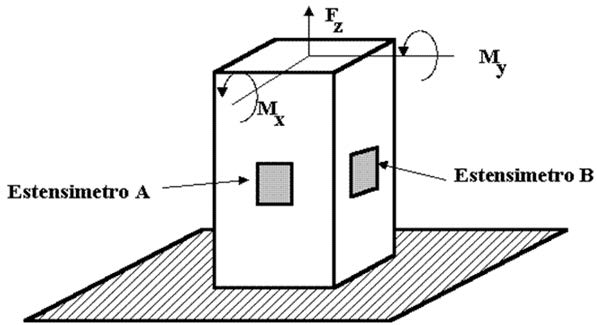
\includegraphics[width=0.3\linewidth]{immagini/23}
	\label{fig:23}
\end{figure}
\newpage
\subparagraph{Misura della Forza $F_z$}\mbox{} \\ 
  		Se si collegano tutti e quattro gli estensimetri e si applica $F_z$, l'uscita per Ponte di Wheatstone per definizione è nulla perché questi misurano tutti la stessa deformazione, la soluzione a questo problema si ottiene considerando solo due estensimetri opposti. 		
  		\begin{figure}[H]
  			\centering
  			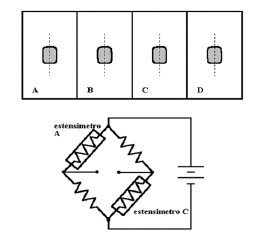
\includegraphics[width=0.4\linewidth]{immagini/screenshot009}
  			\label{fig:screenshot009}
  		\end{figure}  		
  		Per la misura della forza, il Ponte di Wheatstone avrà soltanto due estensimetri sui due rami opposti \textbf{A} e \textbf{C}, le resistenza ulteriori sono resistenze di precisione e di completamento.  		  		
  		\[{E_0\over E_i} = {1\over4}\left({\Delta R_A\over R_A} \textbf{+} {\Delta R_C\over R_C}\right)\]  		
  		\[{\Delta R_A\over R_A} = {\Delta R_C\over R_C} = K\varepsilon = K{F_z\over AE}\]
  		Per cui:
  		\[E_0 = {KE_i\over 2AE} F_z = S_{F_z}F_z \]
  		Similmente alla cella di carico a trazione ma con sensibilità inevitabilmente minore. 		
  		\begin{itemize}
  			\item In presenza di un $M_x$:\[{\Delta R_A\over R_A} = {\Delta R_C\over R_C} = 0 \Rightarrow E_0 = 0\] E l'uscita del ponte è nulla. 
  			\item In presenza di un $M_y$:\[{\Delta R_A\over R_A} = -{\Delta R_C\over R_C} = {6KM_y\over Eh^3} \Rightarrow E_0 = {1\over4}{\Delta R_A\over R_A} + {\Delta R_C\over R_C} = 0\] E l'uscita del ponte è nulla.
  		\end{itemize}
\newpage  	
\subparagraph{Misura del Momento $M_x$}\mbox{} \\
  		Per la misura del momento gli estensimetri che ne misureranno la deformazione saranno quelli contigui \textbf{B} e \textbf{D}, in questo modo quando un estensimetro è in trazione l'altro è in compressione e viceversa. 
\begin{figure}[H]
	\centering
	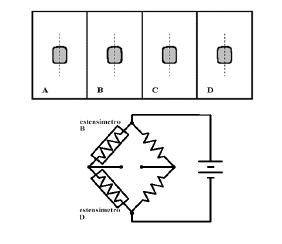
\includegraphics[width=0.4\linewidth]{immagini/screenshot010}
	\label{fig:screenshot010}
\end{figure}
  		\[{E_0\over E_i} = {1\over4}\left({\Delta R_B\over R_B} \textbf{-} {\Delta R_D\over R_D}\right)\]  		
  		\[{\Delta R_B\over R_B} = -{\Delta R_D\over R_D} = K\varepsilon = 6K{M_x\over Eh^3}\]
  		Per cui:
  		\[E_0 = {3KE_i\over Eh^3}M_x = S_{M_x}M_x \] 		
  		\begin{itemize}
  			\item In presenza di una forza $F_z$ lungo l'asse: \[{\Delta R_B\over R_B} = {\Delta R_D\over R_D} = K\varepsilon \Rightarrow E_0 = 0\] E l'uscita del ponte è nulla.
  			\item In presenza di un $M_y$ gli estensimetri \textbf{A} e \textbf{C} si deformano ma non sono all'interno del circuito, quindi:
  			\[{\Delta R_B\over R_B} = {\Delta R_D\over R_D}\simeq0\]
  			E l'uscita del ponte è nulla. 
  		\end{itemize}
\newpage 	
\subparagraph{Misura del Momento $M_y$}\mbox{} \\
  		La misura del momento $M_y$ è analoga a quella di $M_x$ gli estensimetri interessati saranno sempre quelli contigui \textbf{A} e \textbf{C}, in modo da avere un estensimetro in trazione e l'altro in compressione e viceversa.   		
  		\begin{figure}[H]
  			\centering
  			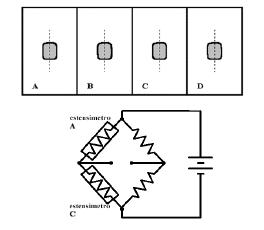
\includegraphics[width=0.4\linewidth]{immagini/screenshot011}
  			\label{fig:screenshot011}
  		\end{figure} 	 		
  		\[{E_0\over E_i} = {1\over4}\left({\Delta R_A\over R_A} \textbf{-} {\Delta R_C\over R_C}\right)\]  		
  		\[{\Delta R_A\over R_A} = -{\Delta R_C\over R_C} = K\varepsilon = 6K{M_y\over Eh^3}\]
  		Per cui:
  		\[E_0 = {3KE_i\over Eh^3}M_y = S_{M_y}M_y \]		
  		\begin{itemize}
  			\item In presenza di una forza $F_z$ lungo l'asse: \[{\Delta R_A\over R_A} = {\Delta R_C\over R_C} = K\varepsilon \Rightarrow E_0 = 0\] E l'uscita del ponte è nulla.
  			\item In presenza di un $M_x$ gli estensimetri \textbf{B} e \textbf{D} si deformano ma non sono all'interno del circuito, quindi:
  			\[{\Delta R_A\over R_A} = {\Delta R_C\over R_C}\simeq0\]
  			E l'uscita del ponte è nulla. 
  		\end{itemize}  		
  		\begin{figure}[H]
  			\centering
  			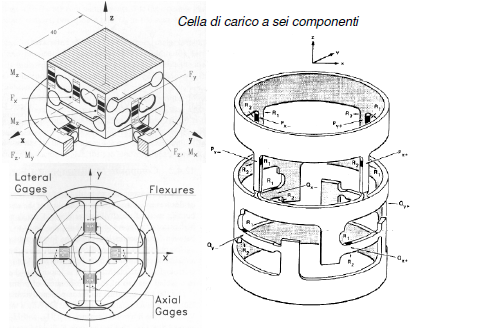
\includegraphics[width=0.5\linewidth]{immagini/screenshot012}
  			\label{fig:screenshot012}
  		\end{figure}
\end{adjustwidth}
\newpage
\subsection{Taratura delle Celle di Carico}	
\subsubsection{Taratura statica}			
\begin{adjustwidth}{2in}{}
  		La taratura statica può essere effettuata per mezzo di:
  		\begin{itemize}
  			\item macchine di trazione alle quali si forniscono forze note;
  			\item una cella di carico tarante in serie ad una cella di carico da tarare (a meno del peso di quella tarante), effettuando una taratura per confronto. 
  			\item utilizzo di pesi noti senza l'ausilio di alcuna cella tarante.\newline 
  			
  			In questo caso in input viene fornita una $F=mg$ dove la $g$ è nota con una sua incertezza, questa dipendente dal luogo in cui si effettua la taratura.  			
  			\begin{figure}[H]
  				\centering
  				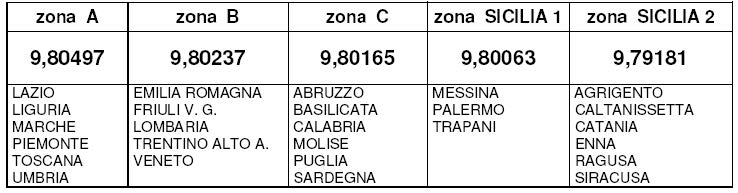
\includegraphics[width=0.6\linewidth]{immagini/24}
  				\label{fig:screenshot013}
  			\end{figure}  			  			
  			E la $m$ con un'incertezza che si basa sul tipo di classe di massa campione acquistata, con distribuzione rettangolare data da $\pm a/\sqrt{3}$ 
\begin{figure}[H]
	\centering
	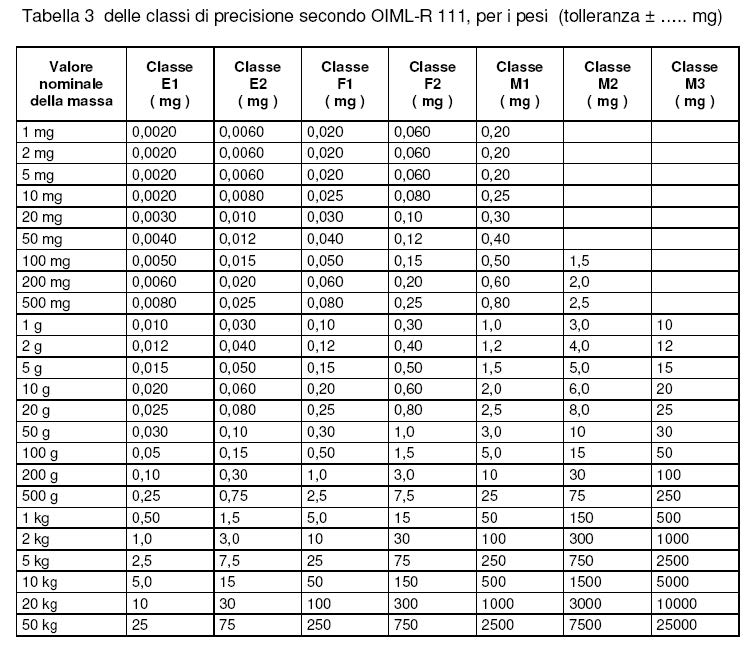
\includegraphics[width=0.6\linewidth]{immagini/25}
	\label{fig:25}
\end{figure}
  		\end{itemize}
\end{adjustwidth}
\newpage
\subsubsection{Taratura dinamica}			
\begin{adjustwidth}{2in}{}
  		La tara tura dinamica prevede la presenza di una cella di carico composta da una massa sismica $M_s$ intelaiata ad una basa insieme ad una molla e ad uno smorzatore. Un accelerometro si preoccuperà infine di misurare l'accelerazione inerziale che lo shaker sta dando al sistema.   		
  		\begin{figure}[H]
  			\centering
  			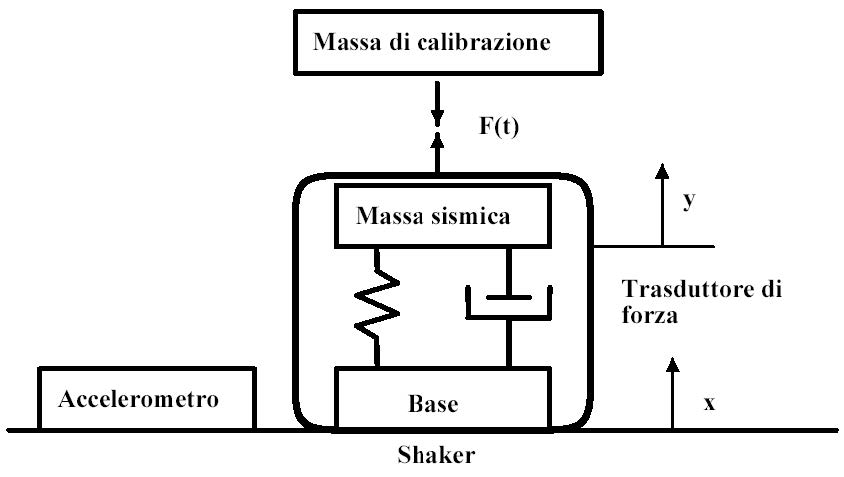
\includegraphics[width=0.5\linewidth]{immagini/26}
  			\label{fig:26}
  		\end{figure}  		   		
  		Si applicano masse di calibrazione $M_c$ e si mette il sistema in vibrazione, si studia l'effetto sismico. \newline 
  		
  		In $x$ è il movimento della shaker mentre in $y$ sarà l'uscita della cella di carico:
  		\[(m_s+m_c)\ddot{y} + c(\dot{y}-\dot{x}) + k(y-x)=0\]
  		In cui \((\dot{y}-\dot{x})\) è la differenza di velocità tra lo shaker e la cella di carico e \((y-x)\) è un termine legato all'elasticità della cella di carico, se non si deformasse non si avrebbero variazioni in $ x $ ed $ y $. \newline 
  		
  		Si sostituisca $z=y-x$:
  		\[(m_s+m_c)\ddot{z} + c\dot{z}+kz=-(m_s+m_c)\ddot{x}\]
  		Se $ E_f $ ed $ E_a $ sono rispettivamente l’uscita in tensione della cella di carico e dell'accelerometro ed $ S_f $ con $ S_a $ le loro sensibilità: 
  		\[E_f = S_f (m_s+m_c)\ddot{x}\]
  		Le grandezze dell'accelerometro si misurano in unità di $g={\ddot{x}\over g}$.
  		\[E_a = S_a{\ddot{x}\over g}\]
  		\[{E_f\over E_a} = {S_f\over S_a }(m_s+m_c)g = {S_f\over S_a }(W_s+W_c)\]
  		Ripetendo lo stesso procedimento variando le masse di calibrazione si giunge ad una retta di regressione:  		
  		\begin{figure}[H]
  			\centering
  			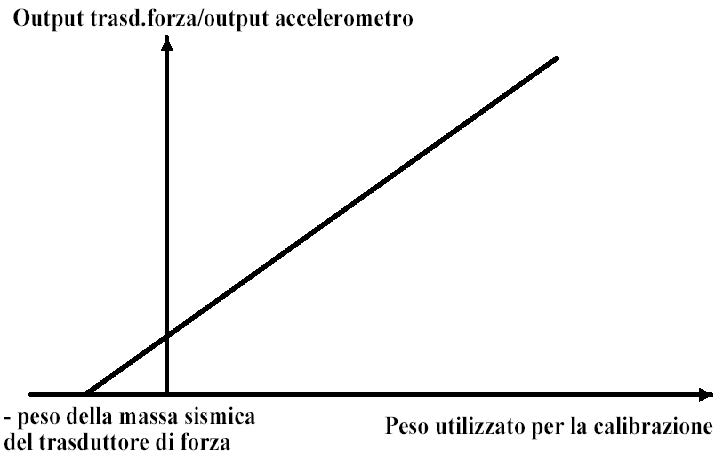
\includegraphics[width=0.3\linewidth]{immagini/27}
  			\label{fig:27}
  		\end{figure}  		  		
  		\[{E_f\over E_a} = {S_f\over S_a }(W_s+W_c)\]
  		Con la quale si può calcolare il coefficiente angolare $s = {S_f\over S_a}$ ed infine giungere alla sensibilità della cella di carico: 
  		\[S_f = s\cdot S_a\]
\end{adjustwidth}
\newpage
\section{Misure di Pressione}		
\begin{adjustwidth}{2in}{}	
  		La pressione è definita come rapporto tra la forza $ F $ e la superficie $ A $ su cui agisce:
  		\[P={F\over A}\]
  		La pressione tanto maggiore quanto minore è la superficie sulla quale agisce una uguale forza. \newline 
  		
  		Come unità di misura ha il pascal: $Pa = {N\over m^2}$. \newline
  		
  		I sensori maggiormente usati per la misura della pressione sono i manometri ad U o a deformazione. \newline 
  		
  		Un manometro può misurare:  		
  		\begin{figure}[H]
  			\centering
  			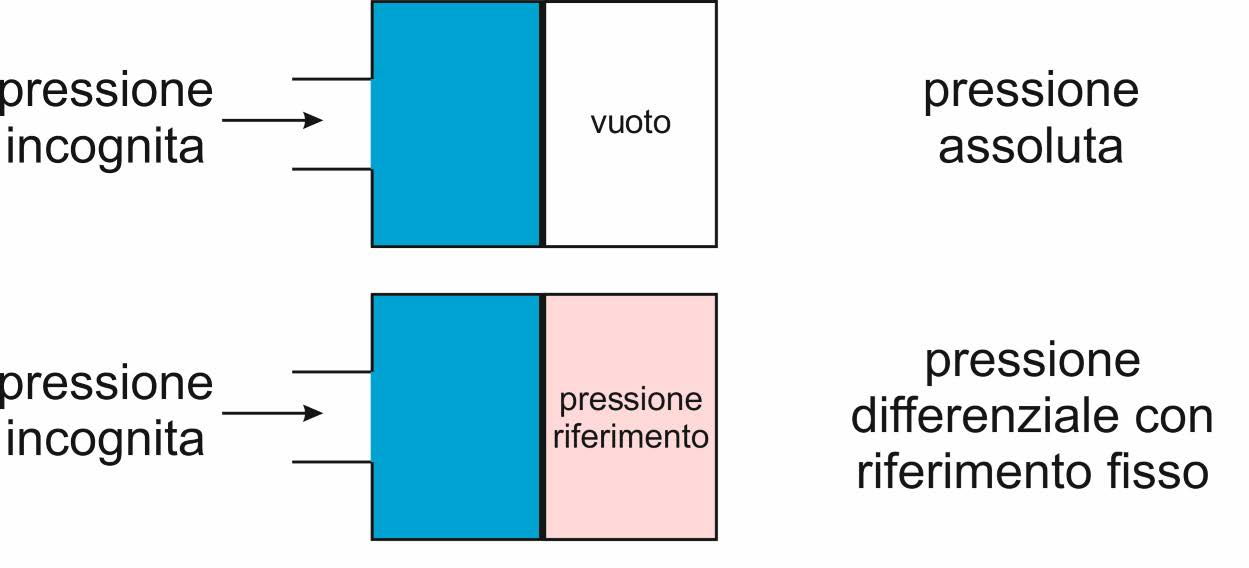
\includegraphics[width=0.3\linewidth]{immagini/p1}
  			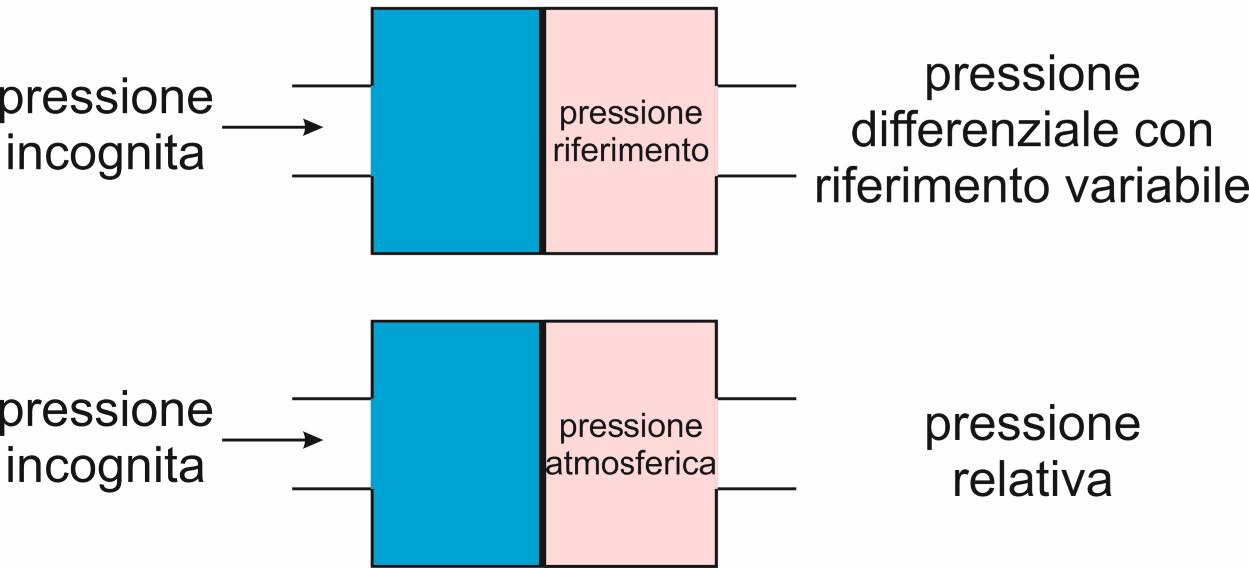
\includegraphics[width=0.3\linewidth]{immagini/p2}
  			\label{fig:p}
  		\end{figure}
  		
\paragraph{Manometro a colonna di liquido}\mbox{} \\
\textbf{Misura della pressione atmosferica} 
		\begin{figure}[H]
			\centering
			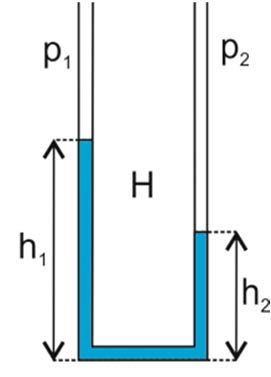
\includegraphics[width=0.2\linewidth]{immagini/p3}
			\label{fig:p3}
		\end{figure}		
  		\[\Delta P \rightarrow \boxed{}\rightarrow H\]
  		Con un tubo ad U contenente mercurio, dopo aver fatto il vuoto il mercurio raggiunge un dislivello $H$ pari a 760 mm equilibrando la pressione atmosferica $1 atm = 76 cmHg$, se $ \gamma_{Hg} = g\rho_{Hg} $:
  		\[p_1 +\gamma_{Hg}h_1 = p_2 +\gamma_{Hg}h_2\]
  		\[p_1-p_2 = \gamma_{Hg}(h_1-h_2) = \gamma_{Hg}(h_1-h_2) \]
  		È uno strumento ad alta precisione di scarso impiego in ambito industriale, utilizzato per la taratura per confronto, ha una bassa risoluzione, è delicato e non adatto a misurare alte pressioni. \newline 
  		
  		La sensibilità di questo strumento è 
  		\[S = {H\over \Delta p} = {1\over\gamma}\]
 \newpage
 		\begin{figure}[H]
 			\centering
 			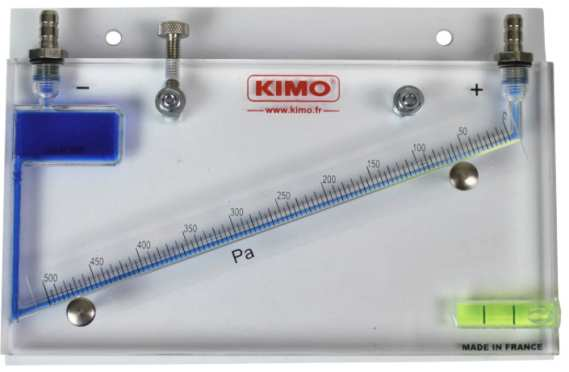
\includegraphics[width=0.5\linewidth]{immagini/p4}
 			\label{fig:p4}
 		\end{figure} 		
  		Per aumentare la sensibilità i manometri da taratura ad U si realizzano con una colonna inclinata di 45\degree piuttosto che verticale, in questo modo: 
  		\[\Delta P = \gamma\cdot H =\gamma\cdot L\sin\alpha \Rightarrow S ={1\over\gamma\sin\alpha} \]
  		Più $\alpha\downarrow$ più $S\uparrow$ ma anche $L\uparrow$ e sono necessari tubi più lunghi.  		
  		
  		Una variazione di sensibilità si ottiene anche variando $\gamma$ ovverosia il liquido misurazione. \newline 
  		
  		È uno strumento che va messo in piano, il sistema ruotato o inclinato introduce grandezze di influenza.  
\end{adjustwidth}
\newpage
\subsection{Manometri a deformazione}		
\begin{adjustwidth}{2in}{}  		
  		 Il manometro a deformazione è formato da un trasduttore primario, chiamato anche elemento elastico questo capace di convertire la pressione in altra grandezza meccanica, generalmente converte il moto rototraslatorio dell'elemento finale in pura rotazione e da un trasduttore secondario il cui compito è quello di fornire in uscita un segnale di natura elettrica che sia funzione dell'output del trasduttore primario. 
  		 \[\text{Pressione}\rightarrow\boxed{I}\rightarrow \text{Deformazione/Spostamento} \rightarrow \boxed{II}\rightarrow\text{Output}\]  		 
\paragraph{Manometro Bourdon - configurazione a C}\mbox{} \\ 
		Prende il nome dall'inventore francese Eugene Bourdon. 
		
		L'elemento deformabile è un tubicino di materiale elastico chiuso all'estremità e  dalla sezione non circolare. 
		
		In dipendenza dei modelli può avere con un angolo di curvatura variabile tra i 150\degree e i 270\degree.		
		\[P\rightarrow\boxed{}\rightarrow \vartheta\]
  		 \begin{figure}[H]
  		 	\centering
  		 	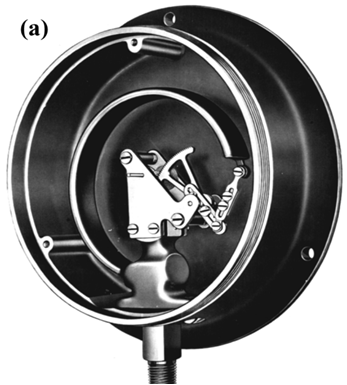
\includegraphics[width=0.2\linewidth]{immagini/manometro3}
  		 	\label{fig:manometro3}
  		 \end{figure}
  		 L'ingresso del manometro viene connesso alla pressione da misurare.
  		 
  		 Il fluido in pressione entra nell'elemento deformabile in modo che l'aumento della stessa tenda a far assumere al tubo una forma circolare, in questo modo la variazione di sezione determina lo spostamento estremale del tubo. 
  		 
  		 L'estremità del tubo si muove di moto rototraslatorio che viene convertito in pura rotazione tramite una movimentazione composta da ruote e pignoni.   		
  		\begin{figure}[H]
  			\centering
  			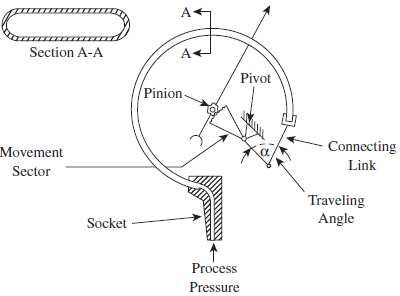
\includegraphics[width=0.5\linewidth]{immagini/manometro1}
  			\label{fig:manometro1}
  		\end{figure}
  	  		Lo spostamento di AA' è funzione:
  		\begin{itemize}
  			\item Dell'angolo totale $\alpha$ noto dall'estensione del tubo
  			\item dalla forma della sezione $a, b$ 
  			\item Da parametri definiti tramite taratura $k, x, y, w$
  			\item Dalla pressione $P$
  			\item Dal materiale utilizzato (modulo di Young $E$)
  			\item Dal raggio di curvatura $R$
  		\end{itemize}
  		Per cui:
  		\[AA' = k{\alpha P\over E}\left(R\over b\right)^x\left(a\over b\right)^y\left(a\over s\right)^w\]
  		LA sensibilità risulta così essere pari a:
  		\[ S = {d\over dP}AA' = k{\alpha\over E}\left(R\over b\right)^x\left(a\over b\right)^y\left(a\over s\right)^w \]
  		Una volta noto lo spostamento $x, y, w$ l'equazione della sensibilità diviene lineare, si nota così che un aumento della stessa lo si ottiene diminuendo $E$, $b$, $s$ spessore e aumentando $a$, e questo spiega inoltre perché la sezione del tubicino debba essere ellittica e non circolare $a\ne b$, in questo modo $b<a$ e la sensibilità ne viene aumentata. 
  		\[S\uparrow~\Leftrightarrow ~ E\downarrow~s\downarrow~b\downarrow~a\uparrow~\alpha\uparrow\quad a<b\]
  		
  		Per incrementare ulteriormente la sensibilità, si passa a configurazioni ad elica o a spirale in modo da far aumentare il parametro $\alpha$.  		
  		\begin{figure}[H]
  			\centering
  			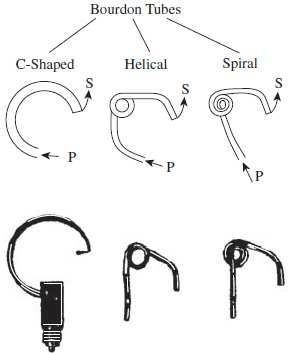
\includegraphics[width=0.3\linewidth]{immagini/manometro4}
  			\label{fig:manometro4}
  		\end{figure}  		
  		Infatti l'elemento deformabile all'interno del manometro può essere di tipo:
  		\begin{itemize}
  			\item \textbf{C} ottenuto curvando l'elemento elastico in modo da formare un segmento circolare. 
  			\item \textbf{Elicoidale} ottenuto aumentando la lunghezza del tubo in modo da ottenere un'elica
  			\item \textbf{Spirale} ottenuto avvolgendo l'elemento elastico per due o tre giri dandone la forma a spirale
  		\end{itemize}
  		I Manometri Bourdon a C sono utilizzati per la misura di elevate pressioni, fino almeno a $700~\text{MPa}$, mentre le altre configurazioni sono urate per misurazioni al di sotto dei $7~\text{kPa}$.  
\newpage 		
\paragraph{Tubo Bourdon a spirale} \mbox{} \\
  		L'elemento a spirale può così essere visto come una serie di elementi a C collegati tra di loro, quando è applicata una pressione la spirale tende a svolgersi e determina uno spostamento maggiore del punto terminale garantendo un movimento di pura rotazione. 
  		\begin{figure}[H]
  			\centering
  			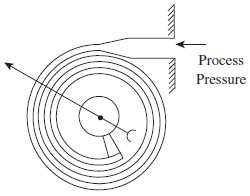
\includegraphics[width=0.3\linewidth]{immagini/manometro5}
  			\label{fig:manometro5}
  		\end{figure} 		
  		Oltre all'aumento della sensibilità dato da un $\alpha$ più elevato si registra anche un aumento dell'accuratezza, questo a causa dell'assenza degli attriti indotti dal meccanismo di conversione del moto del punto finale. \newline 
  		
\paragraph{Tubo Bourdon ad elica} \mbox{} \\
  		L'elemento a spirale determina in questo caso un movimento più ampio della parte terminale del tubicino, si ottiene così un movimento di pura rotazione senza l'ausilio di amplificazione meccanica. 
  		\begin{figure}[H]
  			\centering
  			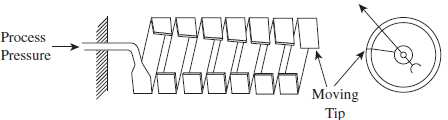
\includegraphics[width=0.3\linewidth]{immagini/manometro6}
  			\label{fig:manometro6}
  		\end{figure}
  		Oltre all'aumento della sensibilità diviene considerevole l'aumento della protezione dello strumento dai sovraccarichi. \newline 
  		
\paragraph{Sezione del tubo} \mbox{} \\
  		Appurato che la sezione del tubo non sia circolare, questa si realizza attraverso equazioni empiriche ed osservazioni pratiche.
  		\begin{figure}[H]
  			\centering
  			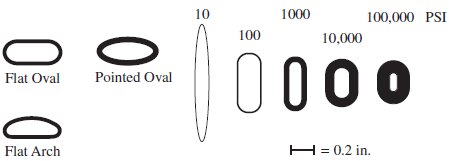
\includegraphics[width=0.3\linewidth]{immagini/manometro7}
  			\label{fig:manometro7}
  		\end{figure}
  		Il manometro Bourdon è caratterizzato da:
  		\begin{itemize}
  			\item Elevata rapidità: $0,1~\text{s}$ al fondo scala
  			\item Limitata linearità: $0.5\%$ del fondo scala
  			\item Presenza di isteresi limitata da trattamenti termici
  			\item Sensibilità alle variazioni di temperatura 
  		\end{itemize}
\newpage  		
\paragraph{Manometro a diaframma} \mbox{} \\
  		Anche in questo caso la pressione provoca la deformazione di un elemento elastico
  		\[\Delta P \rightarrow \boxed{\text{Diaframma}}\underset{\Delta l}{\rightarrow}\boxed{\text{LVDT}}\rightarrow\Delta V\] 
  		A differenza del monometro a C si misura lo spostamento di un diaframma che può essere liscio o corrugato, attraverso un sensori estensimetrici o LVDT. 
  		\begin{figure}[H]
  			\centering
  			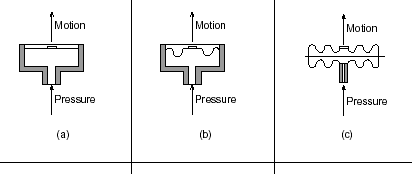
\includegraphics[width=0.3\linewidth]{immagini/manometro8}
  			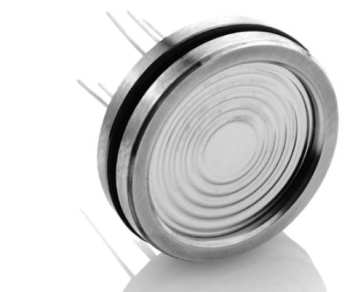
\includegraphics[width=0.2\linewidth]{immagini/manometro9}
  			\label{fig:manometro8}
  			\label{fig:manometro9}
  		\end{figure}
  		\begin{figure}[H]
  			\centering
  			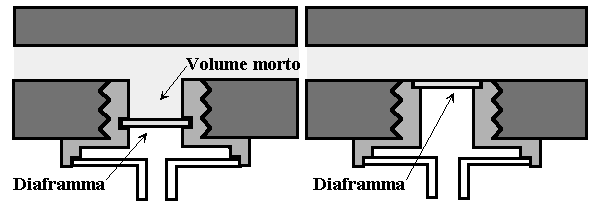
\includegraphics[width=0.5\linewidth]{immagini/manometro10}
  			\label{fig:manometro10}
  		\end{figure}
  		\begin{itemize}[label=\textcolor{green}{\cmark}]
  			\item \textbf{Minore ingombro rispetto al manometro Bourdon}
  			\item \textbf{Curva di taratura nota}
  			\item \textbf{Assenza di un volume morto di fluido}
  				\begin{itemize}[label=\textcolor{green}{\cmark}]
  				\item Aumento della banda passante della catena di misura
  				\end{itemize}
  			\begin{itemize}[label=\textcolor{red}{\xmark}]
  				\item Maggiore dipendenza dell'output da variazioni repentine di temperatura 
  				\item Maggiore sensibilità alle vibrazioni 
  			\end{itemize}
  		\end{itemize}		
 		\begin{itemize}[label=\textcolor{red}{\xmark}]
 			\item \textbf{Isteresi}
 			\item \textbf{Limitata linearità}
 			\item \textbf{Errore di inserzione legato alla resistenza meccanica}
 			
 			Essendo la misura dipendente dalla cedevolezza del diaframma, vincolandolo troppo questo non si sposta e il valore misurano non è corretto. 
 			\item \textbf{Presenza di un volume morto di fluido}
 			
 			Il diaframma non è posto in diretto contatto col fluido
 			
 			Varia il contributo inerziale del sistema di misura: non tanto la massa del diaframma ma la massa di fluido presene nel volume morto
 			\begin{itemize}[label=\textcolor{green}{\cmark}]
 				\item Aumento della capacità termica: minore sensibilità alle variazioni termiche del fluido
 			\end{itemize}
 			\begin{itemize}[label=\textcolor{red}{\xmark}]
 				\item Possibile accumulo di particolato sul diaframma da rimuovere attraverso pulizie periodiche
 				\item Bassa banda passante: se $\Delta P$ varia velocemente, c'è una massa di fluido che si oppone alla vibrazione 
 			\end{itemize}
 		\end{itemize}
\newpage  		
\subparagraph{Diaframma Estensimetrico} \mbox{} \\ 		
 		Uso di estensimetri applicati ad un diaframma liscio che si deforma a cupola. 
 		\begin{figure}[H]
 			\centering
 			\includegraphics[width=0.3\linewidth]{immagini/manometro11}
 			\label{fig:manometro11}
 		\end{figure} 		
 		Analizzando le deformazioni si individuando le zone di massima deformazione della membrana, quelle ovvero dove applicare gli estensimetri.
 		
 		Se $R_0$ è il raggio della membrana ed $r$ è un raggio variabile tra $0$ ed $R_0$, si ottengono:
 		\begin{figure}[H]
 			\centering
 			\includegraphics[width=0.4\linewidth]{immagini/manometro12}
 			\label{fig:manometro12}
 		\end{figure}
 		In cui la curva tratteggiata indice la deformazione tangenziale, mentre quella continua quella radiale. \newline 
 		
 		La deformazione tangenziale $\varepsilon_\theta$ è massima in prossimità del centro, mentre quella radiale $\varepsilon_r$ è massima sulla circonferenza in direzione assiale, si giunge così ad un estensimetro con la seguente configurazione, in cui ci sarà necessario fare attenzione a porre le basette per i collegamenti elettrici in zone in cui le deformazioni sono minime.
 		\begin{figure}[H]
 			\centering
 			\includegraphics[width=0.3\linewidth]{immagini/manometro13}
 			\label{fig:manometro13}
 		\end{figure}
\end{adjustwidth}
\newpage
\subsection{Sistemi di misura per basse pressioni}
\begin{adjustwidth}{2in}{} 
\nointerlineskip\leavevmode
\paragraph{Vacuometro di McLeod} \mbox{} \\
		Utilizzato per pressioni $(0.1\div10)~\text{Pa}$, è costituito da un'ampolla di vetro comunicante con un capillare, una presa di pressione dove effettuare la misura e una pompa manuale o stantuffo.
		
		Il funzionamento si basa sulla compressione da parte mercurio di un campione di gas a partire da una bassa pressione fino al raggiungimento di una pressione sufficientemente elevata da poter essere letta con un manometro. 		 
		\begin{figure}[H]
			\centering
			\includegraphics[width=0.4\linewidth]{immagini/manometro14}
			\label{fig:manometro14}
		\end{figure}				
		\begin{enumerate}
			\item Si porta il mercurio al di sotto dell'ampolla (a) permettendo l'ingresso del gas alla pressione $P_1$
			\item Si spinge lo stantuffo verso il basso andando a limitare un campione del gas nel capillare $A$ ed il mercurio nel capillare $B$.
			
			Entrambi i capillari hanno la stessa sezione.
			\item Si aumenta la pressione fino a portare il livello del mercurio al riferimento 0
			\item Nel capillare $A$ il mercurio rimane ad un livello minore a causa della contropressione del fluido chiuso in $A$.
		\end{enumerate}
		
		Dalla legge di Boyle dei gas perfetti
		\[P_1V_1 = P_2V_2\]
		Dove la pressione all'interno del capillare è
		\[P_2 = P_1 + \rho_{Hg}gh\qquad V_2 = A_ch \]
		In cui $A_c$ è l'area del capillare ed $h$ è il pelo libero del capillare. 
		
		Per cui la pressione incognita sarà
		\[P_1 = \dfrac{P_1+\rho_{Hg}gh}{V_1}A_ch\]
		\[P_1 = \dfrac{\rho_{Hg}gA_ch^2}{V_1-\cancel{A_ch}} \approx \dfrac{\rho_{Hg}gA_ch^2}{V_1}\]
		\begin{itemize}[label=\textcolor{red}{\xmark}]
			\item Strumento assoluto 
			\item Uso delicato, introduzione di errori sistematici
			\item Nel recipiente in cui si vuol misurare la pressione sono immessi vapori di mercurio la cui pressione può falsare la misura
			\item Il vacuometro non misura correttamente la pressione dei vapori che non obbediscono alla legge di Boyle
		\end{itemize}
		
\paragraph{Vacuometro a conducibilità termica} \mbox{} \\
		Dalla teoria cinetica dei gas, per pressioni inferiori ai 100 Pa la conducibilità termica diminuisce linearmente con la pressione.
				
		Il vacuometro a conducibilità termica è costituito da un contenitore collegato al sistema di cui si vuole misurare la pressione. 
		
		All'interno, un filamento di metallo (platino o tungsteno) viene percorso da corrente e viene riscaldato per effetto Joule senza essere portato  all'incandescenza, noto che le perdite di calore per conduzione dipendono dalla pressione, allora la temperatura del filamento dipende dalla quantità di calore che viene scambiata con il gas e, di conseguenza, dalla pressione del gas:
		La misura della pressione diviene ottenibile da una misura diretta della temperatura. \newline 
		
		
\paragraph{Vacuometro a conducibilità termica - a termocoppia} \mbox{} \\
		Realizzato con una termocoppia saldata in un punto del filamento elettrico.
		\begin{figure}[H]
			\centering
			\includegraphics[width=0.5\linewidth]{immagini/manometro15}
			\label{fig:manometro15}
		\end{figure}
		Al variare della pressione del gas, varia il numero di molecole che urta contro il filamento. 
		
		La variazione di temperatura è misurata dalla termocoppia
		
		La risposta dello strumento è legata al gas considerato. 
		
\paragraph{Vacuometro a conducibilità termica - Pirani} \mbox{} \\
 		Utilizza un Ponte di Wheatstone e misura la variazione della resistenza dovuta alla variazione di temperatura in modo che maggiore è la pressione e minore è la temperatura misurata.
\begin{figure}[H]
	\centering
	\label{fig:manometro16}
	\includegraphics[width=0.3\linewidth]{immagini/manometro16}
\end{figure} 		
	 	\begin{itemize}[label=\textcolor{red}{\xmark}]
	 		\item Bassa accuratezza, per misure di basse entità è necessario accettare un grosso errore.
	 	\end{itemize}
	 	\begin{figure}[H]
	 		\centering
	 		\includegraphics[width=0.2\linewidth]{immagini/p5}
	 		\label{fig:p5}
	 	\end{figure}
\newpage	 	
{\LARGE \textbf{NOTE}}
	
	%DA DECOMMENTARE PER AVERE LA VERSIONE STAMPABILE A DUE PAGINE 	
	%	\newpage
	%		\null
	%		\vfill
	%\begin{tcolorbox}[height=4.5cm]
	%	This box has a height of 4.5cm.
	%\end{tcolorbox}
	%		
\end{adjustwidth}
\end{document}